% Standalone Supplementary Material for:
% "CosCert: certified critical values and exact size for long-memory tests of the mean"
\documentclass[final,3p,11pt]{elsarticle}
\usepackage{mathtools}
\usepackage{amsthm}
% p3fonts.tex -- the ONE font set-up shared by the manuscript and by every figure (matplotlib PGF backend, XeLaTeX).
% Latin Modern text with optical sizes (as lmodern does under pdfLaTeX) and Latin Modern Math via unicode-math.
% Fonts are loaded by file name (kpathsea), so no system font cache is consulted or written.
\usepackage{amsmath}
\usepackage{fontspec}
\defaultfontfeatures{Ligatures=TeX}
\setmainfont{lmroman10-regular.otf}[
  UprightFeatures = {SizeFeatures = {
      {Size = -5.5,      Font = lmroman5-regular.otf},
      {Size = 5.5-6.5,   Font = lmroman6-regular.otf},
      {Size = 6.5-7.5,   Font = lmroman7-regular.otf},
      {Size = 7.5-8.5,   Font = lmroman8-regular.otf},
      {Size = 8.5-9.5,   Font = lmroman9-regular.otf},
      {Size = 9.5-11.5,  Font = lmroman10-regular.otf},
      {Size = 11.5-14.5, Font = lmroman12-regular.otf},
      {Size = 14.5-,     Font = lmroman17-regular.otf}}},
  BoldFont = lmroman10-bold.otf,
  BoldFeatures = {SizeFeatures = {
      {Size = -5.5,      Font = lmroman5-bold.otf},
      {Size = 5.5-6.5,   Font = lmroman6-bold.otf},
      {Size = 6.5-7.5,   Font = lmroman7-bold.otf},
      {Size = 7.5-8.5,   Font = lmroman8-bold.otf},
      {Size = 8.5-9.5,   Font = lmroman9-bold.otf},
      {Size = 9.5-11.5,  Font = lmroman10-bold.otf},
      {Size = 11.5-,     Font = lmroman12-bold.otf}}},
  ItalicFont = lmroman10-italic.otf,
  ItalicFeatures = {SizeFeatures = {
      {Size = -7.5,      Font = lmroman7-italic.otf},
      {Size = 7.5-8.5,   Font = lmroman8-italic.otf},
      {Size = 8.5-9.5,   Font = lmroman9-italic.otf},
      {Size = 9.5-11.5,  Font = lmroman10-italic.otf},
      {Size = 11.5-,     Font = lmroman12-italic.otf}}},
  BoldItalicFont = lmroman10-bolditalic.otf]
\setsansfont{lmsans10-regular.otf}[BoldFont = lmsans10-bold.otf, ItalicFont = lmsans10-oblique.otf]
\setmonofont{lmmono10-regular.otf}
\usepackage{unicode-math}
\setmathfont{latinmodern-math.otf}
\setmathfont{latinmodern-math.otf}[version=bold, FakeBold=2]   % bold headings with math (no bold Latin Modern Math exists)

\usepackage{booktabs,array,multirow,makecell,longtable}
\setcounter{LTchunksize}{1000}
\usepackage{graphicx}
\usepackage{xcolor}
\usepackage[font=small,labelfont=bf,skip=5pt]{caption}
\usepackage{microtype}
\usepackage[colorlinks=true,linkcolor=blue!50!black,citecolor=blue!50!black,urlcolor=blue!50!black]{hyperref}
\usepackage[capitalise,nameinlink]{cleveref}
\hypersetup{pdftitle={Supplementary Material -- CosCert: certified critical values and exact size for long-memory tests of the mean},
  pdfauthor={Eslam Ahmed, Mohamed A. El-Beltagy, Ahmed Etman, Sroor M. Elnady}}
\graphicspath{{../figures/}}
\setlength{\emergencystretch}{2em}
\journal{Computational Statistics \& Data Analysis}

% Number sections, tables and figures with S. prefix
\renewcommand{\thesection}{S.\arabic{section}}
\renewcommand{\thetable}{S.\arabic{table}}
\renewcommand{\thefigure}{S.\arabic{figure}}
\renewcommand{\theequation}{S.\arabic{equation}}

% Traceable numbers generated by code/manuscript/make_numbers.py
\makeatletter
\newcommand{\pthreedef}[2]{\expandafter\def\csname p3@#1\endcsname{#2}}
\newcommand{\pthree}[1]{\ifcsname p3@#1\endcsname\csname p3@#1\endcsname\else
  \PackageError{p3numbers}{Undefined number key '#1'}{Run make_numbers.py}\textbf{??#1??}\fi}
\makeatother
% generated by code/manuscript/make_numbers.py -- do not edit
\pthreedef{arfima-trunc}{$1\times10^{-18}$}
\pthreedef{audit-D-hi0-jointz}{3.5}
\pthreedef{audit-D-hi0-max}{4.97}
\pthreedef{audit-D-hi0-maxz}{1.6}
\pthreedef{audit-D-hi0-min}{4.65}
\pthreedef{audit-D-hi0-n}{16}
\pthreedef{audit-D-hi0-rowz}{0.9}
\pthreedef{audit-D-jointz}{5.6}
\pthreedef{audit-D-jointz-rows}{2.8}
\pthreedef{audit-D-nrows}{4}
\pthreedef{audit-apkv-maxrel}{$7.9\times10^{-5}$}
\pthreedef{audit-hi-2se}{0.44}
\pthreedef{audit-hi-disc-max}{$2.0\times10^{0}$}
\pthreedef{audit-hi-neg-design-gt2}{3}
\pthreedef{audit-hi-neg-design-gt3}{0}
\pthreedef{audit-hi-neg-design-max}{5.45}
\pthreedef{audit-hi-neg-design-maxz}{2.08}
\pthreedef{audit-hi-neg-design-min}{4.56}
\pthreedef{audit-hi-neg-gt2se}{29}
\pthreedef{audit-hi-neg-gt3se}{28}
\pthreedef{audit-hi-neg-m1-limit}{3.1}
\pthreedef{audit-hi-neg-m16-T1e3}{3.9}
\pthreedef{audit-hi-neg-m16-T1e4}{5.5}
\pthreedef{audit-hi-neg-m16-T1e5}{7.0}
\pthreedef{audit-hi-neg-m16-fgn}{27.5}
\pthreedef{audit-hi-neg-m16-limit}{29.5}
\pthreedef{audit-hi-neg-max}{29.53}
\pthreedef{audit-hi-neg-maxdev}{24.5}
\pthreedef{audit-hi-neg-maxz}{113}
\pthreedef{audit-hi-neg-min}{3.13}
\pthreedef{audit-hi-neg-n}{80}
\pthreedef{audit-hi-pos-gt01}{58}
\pthreedef{audit-hi-pos-max}{5.34}
\pthreedef{audit-hi-pos-min}{4.65}
\pthreedef{audit-hi-pos-n}{96}
\pthreedef{audit-kpss-tau-05}{5.23}
\pthreedef{audit-kpss-tau-05-exact}{0.1479}
\pthreedef{audit-kpss-tau-05-z}{2.4}
\pthreedef{audit-kpsstau-jointz}{2.5}
\pthreedef{audit-lob-jointz}{1.7}
\pthreedef{audit-lob-sizes}{10.010, 5.023, 2.535, 1.015, 0.525}
\pthreedef{audit-mp-H090-a10}{10.31}
\pthreedef{audit-mp-T1-devmax}{-0.17}
\pthreedef{audit-mp-T1-devmin}{-0.46}
\pthreedef{audit-mp-T1-maxz}{3.8}
\pthreedef{audit-mp-T1-minz}{3.4}
\pthreedef{audit-mp-T3-dev10}{-2.85}
\pthreedef{audit-mp-T3-maxz}{28}
\pthreedef{audit-mp-T3-round-maxshift}{0.05}
\pthreedef{audit-mp-T3-round-mindev}{0.95}
\pthreedef{audit-mp-T3-size05}{2.33}
\pthreedef{audit-mp-neg-max}{-0.02}
\pthreedef{audit-mp-neg-min}{-2.85}
\pthreedef{audit-mp-pos-max}{0.31}
\pthreedef{audit-mp-pos-maxz}{2.94}
\pthreedef{audit-mp-pos-min}{0.03}
\pthreedef{audit-mp-pos-n}{16}
\pthreedef{audit-mp-pos-npos}{16}
\pthreedef{audit-n-A}{83}
\pthreedef{audit-n-AB}{165}
\pthreedef{audit-n-B}{82}
\pthreedef{audit-n-C}{28}
\pthreedef{audit-n-D}{32}
\pthreedef{audit-n-E}{8}
\pthreedef{audit-n-dup}{8}
\pthreedef{audit-n-entries}{241}
\pthreedef{audit-n-sources}{6}
\pthreedef{audit-n-values}{233}
\pthreedef{audit-n-within3}{189}
\pthreedef{bw-50-max-100}{22.3}
\pthreedef{bw-50-max-2000}{12.0}
\pthreedef{bw-50-min-100}{7.2}
\pthreedef{bw-50-min-2000}{5.9}
\pthreedef{bw-65-max-100}{17.8}
\pthreedef{bw-65-max-2000}{7.9}
\pthreedef{bw-65-min-100}{6.6}
\pthreedef{bw-65-min-2000}{5.3}
\pthreedef{bw-80-arfima0-max-500}{9.9}
\pthreedef{bw-80-fgn-maxdev-500}{0.7}
\pthreedef{bw-80-max-100}{16.5}
\pthreedef{bw-80-max-2000}{7.0}
\pthreedef{bw-80-min-100}{5.5}
\pthreedef{bw-80-min-2000}{4.4}
\pthreedef{clip-max}{one}
\pthreedef{clip-ncells}{120}
\pthreedef{clip-nwith}{67}
\pthreedef{clip-rel}{$9\times10^{-17}$}
\pthreedef{dominance-ncells}{120}
\pthreedef{dominance-share}{89}
\pthreedef{e1-slope-maxdev}{0.05}
\pthreedef{e1-tilt-node-ratio-max}{17}
\pthreedef{e1-tilt-node-ratio-min}{1.8}
\pthreedef{e1-width-max-16384}{$1.9\times10^{-6}$}
\pthreedef{e11-n-cat}{6}
\pthreedef{e11-n-rows}{19}
\pthreedef{e2r-maxchange}{$3\times10^{-15}$}
\pthreedef{e2r-n-brackets}{300}
\pthreedef{e2r-n-ok}{300}
\pthreedef{e5-3mom-T1-pp}{1.2}
\pthreedef{e5-T12-cert-s}{0.04}
\pthreedef{e5-T12-cert-width}{$8\times10^{-16}$}
\pthreedef{e5-T12-exact-maxerr}{$4\times10^{-11}$}
\pthreedef{e5-T12-exact-maxs}{$9\times10^{-3}$}
\pthreedef{e5-T3-eig-s}{0.31}
\pthreedef{e5-T3-ifft-s}{975}
\pthreedef{e5-T3-imhof-s}{0.32}
\pthreedef{e5-T3-query-s}{0.06}
\pthreedef{e5-T3-setup-s}{0.37}
\pthreedef{e5-T4-cert-eval-s}{15.7}
\pthreedef{e5-T4-cert-s}{40.5}
\pthreedef{e5-T4-galerkin-err}{$9.5\times10^{-9}$}
\pthreedef{e5-T4-galerkin-s}{0.3}
\pthreedef{e5-T4-ray2048-s}{3049}
\pthreedef{e5-T4-ref-width}{$1.9\times10^{-8}$}
\pthreedef{e5-amort-imhof-s}{4.0}
\pthreedef{e5-amort-m}{10}
\pthreedef{e5-amort-maxdiff}{$6\times10^{-14}$}
\pthreedef{e5-amort-ours-s}{1.1}
\pthreedef{e5-amort-ratio}{3.6}
\pthreedef{e5-approx-maxerr-pp}{5.0}
\pthreedef{e5-env}{12 logical CPUs, Windows 10, Python 3.12.14, R 4.5.3}
\pthreedef{e5-gh-maxdiff-pp}{0.08}
\pthreedef{e5-hbe-err-pp}{1.17}
\pthreedef{e5-lead20-err}{$1.5\times10^{-8}$}
\pthreedef{e5-lpb4-err-pp}{0.23}
\pthreedef{e5-lr-err-pp}{0.88}
\pthreedef{e5-ltz-T1-pp}{1.2}
\pthreedef{e5-n-fail}{4}
\pthreedef{e5-n-impl}{21}
\pthreedef{e5-n-methods}{14}
\pthreedef{e5-n-targets-rows}{92}
\pthreedef{e5-satt-err-pp}{4.6}
\pthreedef{e5-svsaddle-err-pp}{0.19}
\pthreedef{edge-C-0.900}{38.86}
\pthreedef{edge-C-0.950}{69.76}
\pthreedef{edge-C-0.990}{191.0}
\pthreedef{edge-extrap-maxrel}{0.07}
\pthreedef{edge-mu1-share}{81}
\pthreedef{edge-rho-min}{0.23}
\pthreedef{fgn-sn-0.70-500-dev}{$2.4\times10^{-5}$}
\pthreedef{fn-arfima1m-HI16-0.50-50}{1.9}
\pthreedef{fn-arfima1p-HI1-0.50-50}{5.1}
\pthreedef{fn-arfima1p-HI16-0.50-50}{19.1}
\pthreedef{fn-arfima1p-HI16-0.90-50}{12.0}
\pthreedef{fn-arfima1p-HI4-0.70-100}{5.5}
\pthreedef{fn-arfima1p-SN-0.50-50}{7.2}
\pthreedef{fn-arfima1p-SN-0.70-100}{5.5}
\pthreedef{fn-maxdev-2000}{0.05}
\pthreedef{fn-maxdev-pure}{0.54}
\pthreedef{fn-maxdev-small-100}{0.56}
\pthreedef{fx-n-cells}{3\,900}
\pthreedef{g0-max-digits}{15}
\pthreedef{g0-min-digits}{14}
\pthreedef{hi17-R}{100\,000}
\pthreedef{hi17-T5-64-16-plugin}{22.6}
\pthreedef{hi17-maxdiff}{2.0}
\pthreedef{hi17-meandiff}{+0.19}
\pthreedef{hi17-ncells}{144}
\pthreedef{hi17-share-z2}{35}
\pthreedef{hi17-t2-maxz}{2.17}
\pthreedef{hi17-t2-n}{64}
\pthreedef{ledger-n-cv}{245}
\pthreedef{ledger-n-rr}{317}
\pthreedef{mx-0.50-128}{5.0042}
\pthreedef{mx-0.50-64}{5.0167}
\pthreedef{mx-0.90-128}{42.8081}
\pthreedef{mx-0.90-64}{42.8085}
\pthreedef{mx-0.99-128}{79.5227}
\pthreedef{mx-0.99-128-own}{5.00004}
\pthreedef{mx-0.99-128-round}{5.00008}
\pthreedef{mx-0.99-64}{79.5227}
\pthreedef{mx-cv-0.99}{6829.94}
\pthreedef{mx-gap-128}{$4.2\times10^{-3}$}
\pthreedef{mx-gap-128-H}{0.50}
\pthreedef{mx-gap-128-long}{$6.9\times10^{-5}$}
\pthreedef{mx-gap-64}{$1.7\times10^{-2}$}
\pthreedef{mx-gap-64-H}{0.50}
\pthreedef{mx-gap-64-long}{$4.9\times10^{-4}$}
\pthreedef{mx-maxdiff-AB}{$6.7\times10^{-12}$}
\pthreedef{mx-maxdiff-user}{$3.6\times10^{-5}$}
\pthreedef{naive-hi1-0.90}{26.2}
\pthreedef{naive-hi16-0.90}{71.3}
\pthreedef{naive-hi4-0.90}{55.2}
\pthreedef{naive-max-0.90}{71.3}
\pthreedef{naive-min-0.90}{25.6}
\pthreedef{naive-sn-0.70-0.05}{16.5}
\pthreedef{naive-sn-0.90-0.05}{42.8}
\pthreedef{or-inside-pct}{98.9}
\pthreedef{or-maxz}{3.82}
\pthreedef{or-n-cells}{1\,800}
\pthreedef{or-z-mean}{-0.09}
\pthreedef{or-z-sd}{0.99}
\pthreedef{pl-HI4-H05-trunc}{4.6}
\pthreedef{pl-HI4-H05-untrunc}{9.5}
\pthreedef{pl-R}{40\,000}
\pthreedef{pl-ar1m-max-100}{23.5}
\pthreedef{pl-ar1p-max}{4.6}
\pthreedef{pl-ar1p-min}{1.9}
\pthreedef{pl-arfima0-HI16-0.7-100}{11.8}
\pthreedef{pl-arfima0-HI16-0.7-2000}{6.8}
\pthreedef{pl-arfima0-HI16-0.9-100}{17.8}
\pthreedef{pl-arfima0-HI16-0.9-2000}{7.9}
\pthreedef{pl-arfima0-HI4-0.7-100}{10.2}
\pthreedef{pl-arfima0-HI4-0.7-2000}{6.2}
\pthreedef{pl-arfima0-HI4-0.9-100}{15.8}
\pthreedef{pl-arfima0-HI4-0.9-2000}{7.2}
\pthreedef{pl-arfima0-SN-0.7-100}{9.0}
\pthreedef{pl-arfima0-SN-0.7-2000}{5.8}
\pthreedef{pl-arfima0-SN-0.9-100}{13.2}
\pthreedef{pl-arfima0-SN-0.9-2000}{6.4}
\pthreedef{pl-arfima1m-HI16-0.7-100}{14.5}
\pthreedef{pl-arfima1m-HI16-0.7-2000}{7.3}
\pthreedef{pl-arfima1m-HI16-0.9-100}{23.5}
\pthreedef{pl-arfima1m-HI16-0.9-2000}{9.0}
\pthreedef{pl-arfima1m-HI4-0.7-100}{12.3}
\pthreedef{pl-arfima1m-HI4-0.7-2000}{6.4}
\pthreedef{pl-arfima1m-HI4-0.9-100}{20.4}
\pthreedef{pl-arfima1m-HI4-0.9-2000}{8.2}
\pthreedef{pl-arfima1m-SN-0.7-100}{10.3}
\pthreedef{pl-arfima1m-SN-0.7-2000}{5.9}
\pthreedef{pl-arfima1m-SN-0.9-100}{16.4}
\pthreedef{pl-arfima1m-SN-0.9-2000}{7.0}
\pthreedef{pl-arfima1p-HI16-0.7-100}{3.1}
\pthreedef{pl-arfima1p-HI16-0.7-2000}{4.0}
\pthreedef{pl-arfima1p-HI16-0.9-100}{3.4}
\pthreedef{pl-arfima1p-HI16-0.9-2000}{3.7}
\pthreedef{pl-arfima1p-HI4-0.7-100}{3.2}
\pthreedef{pl-arfima1p-HI4-0.7-2000}{4.1}
\pthreedef{pl-arfima1p-HI4-0.9-100}{3.4}
\pthreedef{pl-arfima1p-HI4-0.9-2000}{3.7}
\pthreedef{pl-arfima1p-SN-0.7-100}{3.0}
\pthreedef{pl-arfima1p-SN-0.7-2000}{4.2}
\pthreedef{pl-arfima1p-SN-0.9-100}{3.1}
\pthreedef{pl-arfima1p-SN-0.9-2000}{3.5}
\pthreedef{pl-fgn-HI16-0.7-100}{11.1}
\pthreedef{pl-fgn-HI16-0.7-2000}{6.9}
\pthreedef{pl-fgn-HI16-0.9-100}{15.6}
\pthreedef{pl-fgn-HI16-0.9-2000}{7.8}
\pthreedef{pl-fgn-HI4-0.7-100}{9.7}
\pthreedef{pl-fgn-HI4-0.7-2000}{6.2}
\pthreedef{pl-fgn-HI4-0.9-100}{14.0}
\pthreedef{pl-fgn-HI4-0.9-2000}{7.2}
\pthreedef{pl-fgn-SN-0.7-100}{8.6}
\pthreedef{pl-fgn-SN-0.7-2000}{5.9}
\pthreedef{pl-fgn-SN-0.9-100}{11.8}
\pthreedef{pl-fgn-SN-0.9-2000}{6.5}
\pthreedef{pl-n-pure-cells}{40}
\pthreedef{pl-pure-max-100}{17.8}
\pthreedef{pl-pure-max-2000}{7.9}
\pthreedef{pl-pure-min-100}{5.5}
\pthreedef{pl-pure-min-2000}{5.2}
\pthreedef{pl-share-ewc4-le-sn}{65}
\pthreedef{pl-share-hi1-le-sn}{100}
\pthreedef{pl-share-sn-le-hi4}{100}
\pthreedef{pw-HI1-0.75}{0.354}
\pthreedef{pw-HI16-0.50}{0.775}
\pthreedef{pw-HI16-0.75}{0.770}
\pthreedef{pw-HI16-0.90}{0.758}
\pthreedef{pw-HI4-0.70}{0.687}
\pthreedef{pw-HI4-0.75}{0.685}
\pthreedef{pw-SN-0.50}{0.599}
\pthreedef{pw-SN-0.70}{0.542}
\pthreedef{pw-SN-0.90}{0.491}
\pthreedef{pw-c0-maxdev}{$1.3\times10^{-9}$}
\pthreedef{pw-hi-ewc-maxdiff}{0.002}
\pthreedef{pw-jl-128-512}{$8.0\times10^{-8}$}
\pthreedef{pw-jl-256-512}{$9.0\times10^{-9}$}
\pthreedef{pw-jl-512-1024}{$1.1\times10^{-9}$}
\pthreedef{pw-nct-maxdev}{$2.3\times10^{-13}$}
\pthreedef{pw-nct-ncells}{610}
\pthreedef{pw-vsSN-EWC2-min}{-0.288}
\pthreedef{pw-vsSN-EWC2-npos}{0}
\pthreedef{pw-vsSN-EWC4-min}{-0.037}
\pthreedef{pw-vsSN-EWC4-npos}{304}
\pthreedef{pw-vsSN-EWC8-min}{0.000}
\pthreedef{pw-vsSN-EWC8-npos}{360}
\pthreedef{pw-vsSN-HI1-min}{-0.288}
\pthreedef{pw-vsSN-HI1-npos}{0}
\pthreedef{pw-vsSN-HI2-min}{-0.037}
\pthreedef{pw-vsSN-HI2-npos}{305}
\pthreedef{pw-vsSN-HI4-min}{0.000}
\pthreedef{pw-vsSN-HI4-npos}{360}
\pthreedef{pw-vsSN-ncells}{360}
\pthreedef{pw-z}{0.800}
\pthreedef{rs-maxerr-090-0.01}{0.27}
\pthreedef{rs-maxerr-090-0.05}{0.59}
\pthreedef{rs-maxerr-090-0.10}{0.73}
\pthreedef{rs-maxerr-099-0.05}{1.03}
\pthreedef{rs-sn-0.75-0.05}{7.44}
\pthreedef{rs-sn-0.95-0.05}{9.44}
\pthreedef{rs-surface-K}{7}
\pthreedef{rs-surface-cert-argH}{0.51}
\pthreedef{rs-surface-cert-maxerr}{$2.4\times10^{-4}$}
\pthreedef{rs-surface-cert-ncells}{150}
\pthreedef{rs-surface-cert-ndirect}{82}
\pthreedef{rs-surface-digits}{7}
\pthreedef{rs-surface-fit-maxerr}{$4.0\times10^{-7}$}
\pthreedef{rs-surface-guar-maxerr}{$1.4\times10^{-4}$}
\pthreedef{rs-surface-ncoef}{8}
\pthreedef{sn-bracket-maxerr}{$2.9\times10^{-4}$}
\pthreedef{sn-infl-0.80-0.950}{5.00}
\pthreedef{sn-infl-0.90-0.950}{12.4}
\pthreedef{sn-infl-0.95-0.950}{27.6}
\pthreedef{sn-infl-0.99-0.950}{150}
\pthreedef{sn-max-relwidth}{$1.8\times10^{-5}$}
\pthreedef{sn-n-H}{50}
\pthreedef{sn-n-cells}{300}
\pthreedef{sn-print-maxerr}{0.002}
\pthreedef{sn-q-0.50-0.800}{15.015}
\pthreedef{sn-q-0.50-0.900}{28.331}
\pthreedef{sn-q-0.50-0.950}{45.53}
\pthreedef{sn-q-0.50-0.975}{66.59}
\pthreedef{sn-q-0.50-0.980}{74.19}
\pthreedef{sn-q-0.50-0.990}{100.3}
\pthreedef{sn-q-0.51-0.800}{15.637}
\pthreedef{sn-q-0.51-0.900}{29.58}
\pthreedef{sn-q-0.51-0.950}{47.63}
\pthreedef{sn-q-0.51-0.975}{69.80}
\pthreedef{sn-q-0.51-0.980}{77.82}
\pthreedef{sn-q-0.51-0.990}{105.44}
\pthreedef{sn-q-0.52-0.800}{16.290}
\pthreedef{sn-q-0.52-0.900}{30.885}
\pthreedef{sn-q-0.52-0.950}{49.85}
\pthreedef{sn-q-0.52-0.975}{73.19}
\pthreedef{sn-q-0.52-0.980}{81.6}
\pthreedef{sn-q-0.52-0.990}{110.82}
\pthreedef{sn-q-0.53-0.800}{16.975}
\pthreedef{sn-q-0.53-0.900}{32.260}
\pthreedef{sn-q-0.53-0.950}{52.18}
\pthreedef{sn-q-0.53-0.975}{76.77}
\pthreedef{sn-q-0.53-0.980}{85.68}
\pthreedef{sn-q-0.53-0.990}{116.50}
\pthreedef{sn-q-0.54-0.800}{17.694}
\pthreedef{sn-q-0.54-0.900}{33.71}
\pthreedef{sn-q-0.54-0.950}{54.64}
\pthreedef{sn-q-0.54-0.975}{80.54}
\pthreedef{sn-q-0.54-0.980}{89.94}
\pthreedef{sn-q-0.54-0.990}{122.50}
\pthreedef{sn-q-0.55-0.800}{18.450}
\pthreedef{sn-q-0.55-0.900}{35.23}
\pthreedef{sn-q-0.55-0.950}{57.23}
\pthreedef{sn-q-0.55-0.975}{84.52}
\pthreedef{sn-q-0.55-0.980}{94.45}
\pthreedef{sn-q-0.55-0.990}{128.9}
\pthreedef{sn-q-0.56-0.800}{19.245}
\pthreedef{sn-q-0.56-0.900}{36.834}
\pthreedef{sn-q-0.56-0.950}{59.96}
\pthreedef{sn-q-0.56-0.975}{88.73}
\pthreedef{sn-q-0.56-0.980}{99.21}
\pthreedef{sn-q-0.56-0.990}{135.58}
\pthreedef{sn-q-0.57-0.800}{20.082}
\pthreedef{sn-q-0.57-0.900}{38.526}
\pthreedef{sn-q-0.57-0.950}{62.848}
\pthreedef{sn-q-0.57-0.975}{93.18}
\pthreedef{sn-q-0.57-0.980}{104.25}
\pthreedef{sn-q-0.57-0.990}{142.71}
\pthreedef{sn-q-0.58-0.800}{20.964}
\pthreedef{sn-q-0.58-0.900}{40.312}
\pthreedef{sn-q-0.58-0.950}{65.901}
\pthreedef{sn-q-0.58-0.975}{97.90}
\pthreedef{sn-q-0.58-0.980}{109.58}
\pthreedef{sn-q-0.58-0.990}{150.27}
\pthreedef{sn-q-0.59-0.800}{21.894}
\pthreedef{sn-q-0.59-0.900}{42.199}
\pthreedef{sn-q-0.59-0.950}{69.132}
\pthreedef{sn-q-0.59-0.975}{102.893}
\pthreedef{sn-q-0.59-0.980}{115.24}
\pthreedef{sn-q-0.59-0.990}{158.30}
\pthreedef{sn-q-0.60-0.800}{22.876}
\pthreedef{sn-q-0.60-0.900}{44.195}
\pthreedef{sn-q-0.60-0.950}{72.555}
\pthreedef{sn-q-0.60-0.975}{108.194}
\pthreedef{sn-q-0.60-0.980}{121.25}
\pthreedef{sn-q-0.60-0.990}{166.84}
\pthreedef{sn-q-0.61-0.800}{23.9148}
\pthreedef{sn-q-0.61-0.900}{46.308}
\pthreedef{sn-q-0.61-0.950}{76.185}
\pthreedef{sn-q-0.61-0.975}{113.82}
\pthreedef{sn-q-0.61-0.980}{127.635}
\pthreedef{sn-q-0.61-0.990}{175.92}
\pthreedef{sn-q-0.62-0.800}{25.0137}
\pthreedef{sn-q-0.62-0.900}{48.549}
\pthreedef{sn-q-0.62-0.950}{80.040}
\pthreedef{sn-q-0.62-0.975}{119.811}
\pthreedef{sn-q-0.62-0.980}{134.43}
\pthreedef{sn-q-0.62-0.990}{185.588}
\pthreedef{sn-q-0.63-0.800}{26.178}
\pthreedef{sn-q-0.63-0.900}{50.927}
\pthreedef{sn-q-0.63-0.950}{84.137}
\pthreedef{sn-q-0.63-0.975}{126.185}
\pthreedef{sn-q-0.63-0.980}{141.66}
\pthreedef{sn-q-0.63-0.990}{195.90}
\pthreedef{sn-q-0.64-0.800}{27.414}
\pthreedef{sn-q-0.64-0.900}{53.454}
\pthreedef{sn-q-0.64-0.950}{88.50}
\pthreedef{sn-q-0.64-0.975}{132.979}
\pthreedef{sn-q-0.64-0.980}{149.37}
\pthreedef{sn-q-0.64-0.990}{206.92}
\pthreedef{sn-q-0.65-0.800}{28.726}
\pthreedef{sn-q-0.65-0.900}{56.144}
\pthreedef{sn-q-0.65-0.950}{93.147}
\pthreedef{sn-q-0.65-0.975}{140.231}
\pthreedef{sn-q-0.65-0.980}{157.608}
\pthreedef{sn-q-0.65-0.990}{218.70}
\pthreedef{sn-q-0.66-0.800}{30.123}
\pthreedef{sn-q-0.66-0.900}{59.010}
\pthreedef{sn-q-0.66-0.950}{98.110}
\pthreedef{sn-q-0.66-0.975}{147.98}
\pthreedef{sn-q-0.66-0.980}{166.417}
\pthreedef{sn-q-0.66-0.990}{231.309}
\pthreedef{sn-q-0.67-0.800}{31.6118}
\pthreedef{sn-q-0.67-0.900}{62.0706}
\pthreedef{sn-q-0.67-0.950}{103.415}
\pthreedef{sn-q-0.67-0.975}{156.283}
\pthreedef{sn-q-0.67-0.980}{175.852}
\pthreedef{sn-q-0.67-0.990}{244.8}
\pthreedef{sn-q-0.68-0.800}{33.2009}
\pthreedef{sn-q-0.68-0.900}{65.343}
\pthreedef{sn-q-0.68-0.950}{109.096}
\pthreedef{sn-q-0.68-0.975}{165.18}
\pthreedef{sn-q-0.68-0.980}{185.974}
\pthreedef{sn-q-0.68-0.990}{259.365}
\pthreedef{sn-q-0.69-0.800}{34.9003}
\pthreedef{sn-q-0.69-0.900}{68.8475}
\pthreedef{sn-q-0.69-0.950}{115.191}
\pthreedef{sn-q-0.69-0.975}{174.74}
\pthreedef{sn-q-0.69-0.980}{196.85}
\pthreedef{sn-q-0.69-0.990}{275.00}
\pthreedef{sn-q-0.70-0.800}{36.7212}
\pthreedef{sn-q-0.70-0.900}{72.6087}
\pthreedef{sn-q-0.70-0.950}{121.741}
\pthreedef{sn-q-0.70-0.975}{185.034}
\pthreedef{sn-q-0.70-0.980}{208.564}
\pthreedef{sn-q-0.70-0.990}{291.854}
\pthreedef{sn-q-0.71-0.800}{38.6761}
\pthreedef{sn-q-0.71-0.900}{76.6533}
\pthreedef{sn-q-0.71-0.950}{128.795}
\pthreedef{sn-q-0.71-0.975}{196.131}
\pthreedef{sn-q-0.71-0.980}{221.199}
\pthreedef{sn-q-0.71-0.990}{310.060}
\pthreedef{sn-q-0.72-0.800}{40.7796}
\pthreedef{sn-q-0.72-0.900}{81.012}
\pthreedef{sn-q-0.72-0.950}{136.408}
\pthreedef{sn-q-0.72-0.975}{208.123}
\pthreedef{sn-q-0.72-0.980}{234.860}
\pthreedef{sn-q-0.72-0.990}{329.767}
\pthreedef{sn-q-0.73-0.800}{43.0482}
\pthreedef{sn-q-0.73-0.900}{85.7201}
\pthreedef{sn-q-0.73-0.950}{144.643}
\pthreedef{sn-q-0.73-0.975}{221.112}
\pthreedef{sn-q-0.73-0.980}{249.663}
\pthreedef{sn-q-0.73-0.990}{351.148}
\pthreedef{sn-q-0.74-0.800}{45.5011}
\pthreedef{sn-q-0.74-0.900}{90.8185}
\pthreedef{sn-q-0.74-0.950}{153.573}
\pthreedef{sn-q-0.74-0.975}{235.217}
\pthreedef{sn-q-0.74-0.980}{265.743}
\pthreedef{sn-q-0.74-0.990}{374.40}
\pthreedef{sn-q-0.75-0.800}{48.1606}
\pthreedef{sn-q-0.75-0.900}{96.3545}
\pthreedef{sn-q-0.75-0.950}{163.284}
\pthreedef{sn-q-0.75-0.975}{250.574}
\pthreedef{sn-q-0.75-0.980}{283.259}
\pthreedef{sn-q-0.75-0.990}{399.760}
\pthreedef{sn-q-0.76-0.800}{51.0525}
\pthreedef{sn-q-0.76-0.900}{102.383}
\pthreedef{sn-q-0.76-0.950}{173.87}
\pthreedef{sn-q-0.76-0.975}{267.343}
\pthreedef{sn-q-0.76-0.980}{302.392}
\pthreedef{sn-q-0.76-0.990}{427.493}
\pthreedef{sn-q-0.77-0.800}{54.2074}
\pthreedef{sn-q-0.77-0.900}{108.970}
\pthreedef{sn-q-0.77-0.950}{185.459}
\pthreedef{sn-q-0.77-0.975}{285.711}
\pthreedef{sn-q-0.77-0.980}{323.358}
\pthreedef{sn-q-0.77-0.990}{457.92}
\pthreedef{sn-q-0.78-0.800}{57.6612}
\pthreedef{sn-q-0.78-0.900}{116.191}
\pthreedef{sn-q-0.78-0.950}{198.177}
\pthreedef{sn-q-0.78-0.975}{305.901}
\pthreedef{sn-q-0.78-0.980}{346.412}
\pthreedef{sn-q-0.78-0.990}{491.410}
\pthreedef{sn-q-0.79-0.800}{61.4568}
\pthreedef{sn-q-0.79-0.900}{124.138}
\pthreedef{sn-q-0.79-0.950}{212.192}
\pthreedef{sn-q-0.79-0.975}{328.177}
\pthreedef{sn-q-0.79-0.980}{371.858}
\pthreedef{sn-q-0.79-0.990}{528.417}
\pthreedef{sn-q-0.80-0.800}{65.6455}
\pthreedef{sn-q-0.80-0.900}{132.920}
\pthreedef{sn-q-0.80-0.950}{227.701}
\pthreedef{sn-q-0.80-0.975}{352.856}
\pthreedef{sn-q-0.80-0.980}{400.059}
\pthreedef{sn-q-0.80-0.990}{569.48}
\pthreedef{sn-q-0.81-0.800}{70.2897}
\pthreedef{sn-q-0.81-0.900}{142.670}
\pthreedef{sn-q-0.81-0.950}{244.940}
\pthreedef{sn-q-0.81-0.975}{380.323}
\pthreedef{sn-q-0.81-0.980}{431.456}
\pthreedef{sn-q-0.81-0.990}{615.24}
\pthreedef{sn-q-0.82-0.800}{75.4654}
\pthreedef{sn-q-0.82-0.900}{153.550}
\pthreedef{sn-q-0.82-0.950}{264.202}
\pthreedef{sn-q-0.82-0.975}{411.046}
\pthreedef{sn-q-0.82-0.980}{466.589}
\pthreedef{sn-q-0.82-0.990}{666.495}
\pthreedef{sn-q-0.83-0.800}{81.2666}
\pthreedef{sn-q-0.83-0.900}{165.761}
\pthreedef{sn-q-0.83-0.950}{285.846}
\pthreedef{sn-q-0.83-0.975}{445.607}
\pthreedef{sn-q-0.83-0.980}{506.124}
\pthreedef{sn-q-0.83-0.990}{724.235}
\pthreedef{sn-q-0.84-0.800}{87.8108}
\pthreedef{sn-q-0.84-0.900}{179.553}
\pthreedef{sn-q-0.84-0.950}{310.321}
\pthreedef{sn-q-0.84-0.975}{484.732}
\pthreedef{sn-q-0.84-0.980}{550.894}
\pthreedef{sn-q-0.84-0.990}{789.686}
\pthreedef{sn-q-0.85-0.800}{95.2468}
\pthreedef{sn-q-0.85-0.900}{195.244}
\pthreedef{sn-q-0.85-0.950}{338.197}
\pthreedef{sn-q-0.85-0.975}{529.341}
\pthreedef{sn-q-0.85-0.980}{601.96}
\pthreedef{sn-q-0.85-0.990}{864.40}
\pthreedef{sn-q-0.86-0.800}{103.766}
\pthreedef{sn-q-0.86-0.900}{213.240}
\pthreedef{sn-q-0.86-0.950}{370.206}
\pthreedef{sn-q-0.86-0.975}{580.615}
\pthreedef{sn-q-0.86-0.980}{660.666}
\pthreedef{sn-q-0.86-0.990}{950.40}
\pthreedef{sn-q-0.87-0.800}{113.619}
\pthreedef{sn-q-0.87-0.900}{234.077}
\pthreedef{sn-q-0.87-0.950}{407.305}
\pthreedef{sn-q-0.87-0.975}{640.103}
\pthreedef{sn-q-0.87-0.980}{728.801}
\pthreedef{sn-q-0.87-0.990}{1050.28}
\pthreedef{sn-q-0.88-0.800}{125.138}
\pthreedef{sn-q-0.88-0.900}{258.466}
\pthreedef{sn-q-0.88-0.950}{450.772}
\pthreedef{sn-q-0.88-0.975}{709.868}
\pthreedef{sn-q-0.88-0.980}{808.730}
\pthreedef{sn-q-0.88-0.990}{1167.55}
\pthreedef{sn-q-0.89-0.800}{138.780}
\pthreedef{sn-q-0.89-0.900}{287.377}
\pthreedef{sn-q-0.89-0.950}{502.349}
\pthreedef{sn-q-0.89-0.975}{792.723}
\pthreedef{sn-q-0.89-0.980}{903.683}
\pthreedef{sn-q-0.89-0.990}{1306.98}
\pthreedef{sn-q-0.90-0.800}{155.181}
\pthreedef{sn-q-0.90-0.900}{322.168}
\pthreedef{sn-q-0.90-0.950}{564.474}
\pthreedef{sn-q-0.90-0.975}{892.607}
\pthreedef{sn-q-0.90-0.980}{1018.18}
\pthreedef{sn-q-0.90-0.990}{1475.24}
\pthreedef{sn-q-0.91-0.800}{175.261}
\pthreedef{sn-q-0.91-0.900}{364.802}
\pthreedef{sn-q-0.91-0.950}{640.669}
\pthreedef{sn-q-0.91-0.975}{1015.21}
\pthreedef{sn-q-0.91-0.980}{1158.76}
\pthreedef{sn-q-0.91-0.990}{1681.98}
\pthreedef{sn-q-0.92-0.800}{200.401}
\pthreedef{sn-q-0.92-0.900}{418.222}
\pthreedef{sn-q-0.92-0.950}{736.219}
\pthreedef{sn-q-0.92-0.975}{1169.08}
\pthreedef{sn-q-0.92-0.980}{1335.22}
\pthreedef{sn-q-0.92-0.990}{1941.67}
\pthreedef{sn-q-0.93-0.800}{232.768}
\pthreedef{sn-q-0.93-0.900}{487.055}
\pthreedef{sn-q-0.93-0.950}{859.428}
\pthreedef{sn-q-0.93-0.975}{1367.62}
\pthreedef{sn-q-0.93-0.980}{1562.97}
\pthreedef{sn-q-0.93-0.990}{2277.03}
\pthreedef{sn-q-0.94-0.800}{275.979}
\pthreedef{sn-q-0.94-0.900}{579.011}
\pthreedef{sn-q-0.94-0.950}{1024.13}
\pthreedef{sn-q-0.94-0.975}{1633.20}
\pthreedef{sn-q-0.94-0.980}{1867.67}
\pthreedef{sn-q-0.94-0.990}{2725.97}
\pthreedef{sn-q-0.95-0.800}{336.540}
\pthreedef{sn-q-0.95-0.900}{707.966}
\pthreedef{sn-q-0.95-0.950}{1255.25}
\pthreedef{sn-q-0.95-0.975}{2006.07}
\pthreedef{sn-q-0.95-0.980}{2295.54}
\pthreedef{sn-q-0.95-0.990}{3356.71}
\pthreedef{sn-q-0.96-0.800}{427.463}
\pthreedef{sn-q-0.96-0.900}{901.677}
\pthreedef{sn-q-0.96-0.950}{1602.61}
\pthreedef{sn-q-0.96-0.975}{2566.74}
\pthreedef{sn-q-0.96-0.980}{2939.01}
\pthreedef{sn-q-0.96-0.990}{4305.69}
\pthreedef{sn-q-0.97-0.800}{579.114}
\pthreedef{sn-q-0.97-0.900}{1224.91}
\pthreedef{sn-q-0.97-0.950}{2182.46}
\pthreedef{sn-q-0.97-0.975}{3503.06}
\pthreedef{sn-q-0.97-0.980}{4013.75}
\pthreedef{sn-q-0.97-0.990}{5891.27}
\pthreedef{sn-q-0.98-0.800}{882.586}
\pthreedef{sn-q-0.98-0.900}{1871.95}
\pthreedef{sn-q-0.98-0.950}{3343.60}
\pthreedef{sn-q-0.98-0.975}{5378.61}
\pthreedef{sn-q-0.98-0.980}{6166.76}
\pthreedef{sn-q-0.98-0.990}{9068.55}
\pthreedef{sn-q-0.99-0.800}{1793.35}
\pthreedef{sn-q-0.99-0.900}{3814.26}
\pthreedef{sn-q-0.99-0.950}{6829.94}
\pthreedef{sn-q-0.99-0.975}{11011.2}
\pthreedef{sn-q-0.99-0.980}{12633.1}
\pthreedef{sn-q-0.99-0.990}{18613.1}
\pthreedef{sn-tinfl-0.80-0.950}{2.24}
\pthreedef{sn-tinfl-0.90-0.950}{3.52}
\pthreedef{sn-tinfl-0.95-0.950}{5.25}
\pthreedef{sn-tinfl-0.99-0.950}{12.2}
\pthreedef{val-R}{200\,000}
\pthreedef{val-n-cells}{192}
\pthreedef{val-n-inside}{191}
\pthreedef{val-z-mean}{0.08}
\pthreedef{val-z-sd}{0.97}


\usepackage{placeins}
\renewcommand{\topfraction}{0.9}\renewcommand{\bottomfraction}{0.6}\renewcommand{\textfraction}{0.07}
\renewcommand{\floatpagefraction}{0.75}\setcounter{topnumber}{3}\setcounter{bottomnumber}{2}\setcounter{totalnumber}{5}
\newsavebox{\fixcitebox}
\newcommand{\fixcite}[1]{\sbox{\fixcitebox}{[00]}\makebox[\wd\fixcitebox][l]{\citep{#1}}}
\newcommand{\CosCert}{CosCert}
\newcommand{\E}{\mathbb E}
\newcommand{\Bt}{\tilde B_H}

\begin{document}
\begin{frontmatter}
\title{Supplementary Material for:\\\CosCert: certified critical values and exact size\\ for long-memory tests of the mean}
\author[a]{Eslam Ahmed\corref{cor1}}
\ead{eslamahmed@eng.cu.edu.eg}
\author[a]{Mohamed A. El-Beltagy}
\author[a]{Ahmed Etman}
\author[b,c]{Sroor M. Elnady}
\cortext[cor1]{Corresponding author}
\affiliation[a]{organization={Department of Engineering Mathematics and Physics, Faculty of Engineering, Cairo University},city={Giza},postcode={12613},country={Egypt}}
\affiliation[b]{organization={School of Aeronautics and Astronautics, Zhejiang University},city={Hangzhou},postcode={310027},country={China}}
\affiliation[c]{organization={Center for Research on Microgrids (CROM), Huanjiang Laboratory},city={Zhuji, Shaoxing},postcode={311800},country={China}}
\end{frontmatter}

\noindent This document provides certified reference tables, extended finite-sample and bandwidth-sensitivity tables, the full 233-value literature audit ledger and the validation and reproducibility verification package accompanying the main manuscript. Every number and table is generated directly from the archival result files by \texttt{code/manuscript/make\_numbers.py}.

% ============================================================================ S.1
\section{Certified critical-value tables}\label{supp:tables}

\Cref{tab:sncvfull} gives the certified quantiles $q_p(H)$ of the Bartlett/self-normalised limit $T_H$ at all \pthree{sn-n-H} values of $H\in\{0.50,0.51,\dots,0.99\}$ and six probability levels; each printed entry is the correctly rounded value of every point in its certified enclosure. \Cref{tab:fixedfull} gives the certified two-sided $5\,\%$ critical values of the fixed-$m$ periodogram statistic \citep{HI17} and the equal-weighted cosine (EWC) statistic \citep{LLSW18} on a $0.05$ grid of $H$ (plus $H=0.99$); all \pthree{fx-n-cells} certified values at $10$, $5$ and $1\,\%$ on $H=0.50,0.51,\dots,0.99$ are provided in \texttt{results/E2\_sn\_critical\_values.json} and \texttt{results/E2b\_fixed\_*.json}.

{\small\setlength{\tabcolsep}{5pt}
\begin{longtable}{@{}lrrrrrr@{}}
\caption{Certified Bartlett quantiles for all tabulated Hurst indices and probability levels.}\label{tab:sncvfull}\\\toprule
$H$ & $q_{0.80}$ & $q_{0.90}$ & $q_{0.95}$ & $q_{0.975}$ & $q_{0.98}$ & $q_{0.99}$\\\midrule\endfirsthead
\caption[]{(continued)}\\\toprule $H$ & $q_{0.80}$ & $q_{0.90}$ & $q_{0.95}$ & $q_{0.975}$ & $q_{0.98}$ & $q_{0.99}$\\\midrule\endhead
\midrule\multicolumn{7}{r@{}}{\footnotesize\itshape continued on the next page}\\\endfoot
\bottomrule\endlastfoot
0.50 & 15.015 & 28.331 & 45.53 & 66.59 & 74.19 & 100.3\\
0.51 & 15.637 & 29.58 & 47.63 & 69.80 & 77.82 & 105.44\\
0.52 & 16.290 & 30.885 & 49.85 & 73.19 & 81.6 & 110.82\\
0.53 & 16.975 & 32.260 & 52.18 & 76.77 & 85.68 & 116.50\\
0.54 & 17.694 & 33.71 & 54.64 & 80.54 & 89.94 & 122.50\\
0.55 & 18.450 & 35.23 & 57.23 & 84.52 & 94.45 & 128.9\\
0.56 & 19.245 & 36.834 & 59.96 & 88.73 & 99.21 & 135.58\\
0.57 & 20.082 & 38.526 & 62.848 & 93.18 & 104.25 & 142.71\\
0.58 & 20.964 & 40.312 & 65.901 & 97.90 & 109.58 & 150.27\\
0.59 & 21.894 & 42.199 & 69.132 & 102.893 & 115.24 & 158.30\\
0.60 & 22.876 & 44.195 & 72.555 & 108.194 & 121.25 & 166.84\\
0.61 & 23.9148 & 46.308 & 76.185 & 113.82 & 127.635 & 175.92\\
0.62 & 25.0137 & 48.549 & 80.040 & 119.811 & 134.43 & 185.588\\
0.63 & 26.178 & 50.927 & 84.137 & 126.185 & 141.66 & 195.90\\
0.64 & 27.414 & 53.454 & 88.50 & 132.979 & 149.37 & 206.92\\
0.65 & 28.726 & 56.144 & 93.147 & 140.231 & 157.608 & 218.70\\
0.66 & 30.123 & 59.010 & 98.110 & 147.98 & 166.417 & 231.309\\
0.67 & 31.6118 & 62.0706 & 103.415 & 156.283 & 175.852 & 244.8\\
0.68 & 33.2009 & 65.343 & 109.096 & 165.18 & 185.974 & 259.365\\
0.69 & 34.9003 & 68.8475 & 115.191 & 174.74 & 196.85 & 275.00\\
0.70 & 36.7212 & 72.6087 & 121.741 & 185.034 & 208.564 & 291.854\\
0.71 & 38.6761 & 76.6533 & 128.795 & 196.131 & 221.199 & 310.060\\
0.72 & 40.7796 & 81.012 & 136.408 & 208.123 & 234.860 & 329.767\\
0.73 & 43.0482 & 85.7201 & 144.643 & 221.112 & 249.663 & 351.148\\
0.74 & 45.5011 & 90.8185 & 153.573 & 235.217 & 265.743 & 374.40\\
0.75 & 48.1606 & 96.3545 & 163.284 & 250.574 & 283.259 & 399.760\\
0.76 & 51.0525 & 102.383 & 173.87 & 267.343 & 302.392 & 427.493\\
0.77 & 54.2074 & 108.970 & 185.459 & 285.711 & 323.358 & 457.92\\
0.78 & 57.6612 & 116.191 & 198.177 & 305.901 & 346.412 & 491.410\\
0.79 & 61.4568 & 124.138 & 212.192 & 328.177 & 371.858 & 528.417\\
0.80 & 65.6455 & 132.920 & 227.701 & 352.856 & 400.059 & 569.48\\
0.81 & 70.2897 & 142.670 & 244.940 & 380.323 & 431.456 & 615.24\\
0.82 & 75.4654 & 153.550 & 264.202 & 411.046 & 466.589 & 666.495\\
0.83 & 81.2666 & 165.761 & 285.846 & 445.607 & 506.124 & 724.235\\
0.84 & 87.8108 & 179.553 & 310.321 & 484.732 & 550.894 & 789.686\\
0.85 & 95.2468 & 195.244 & 338.197 & 529.341 & 601.96 & 864.40\\
0.86 & 103.766 & 213.240 & 370.206 & 580.615 & 660.666 & 950.40\\
0.87 & 113.619 & 234.077 & 407.305 & 640.103 & 728.801 & 1050.28\\
0.88 & 125.138 & 258.466 & 450.772 & 709.868 & 808.730 & 1167.55\\
0.89 & 138.780 & 287.377 & 502.349 & 792.723 & 903.683 & 1306.98\\
0.90 & 155.181 & 322.168 & 564.474 & 892.607 & 1018.18 & 1475.24\\
0.91 & 175.261 & 364.802 & 640.669 & 1015.21 & 1158.76 & 1681.98\\
0.92 & 200.401 & 418.222 & 736.219 & 1169.08 & 1335.22 & 1941.67\\
0.93 & 232.768 & 487.055 & 859.428 & 1367.62 & 1562.97 & 2277.03\\
0.94 & 275.979 & 579.011 & 1024.13 & 1633.20 & 1867.67 & 2725.97\\
0.95 & 336.540 & 707.966 & 1255.25 & 2006.07 & 2295.54 & 3356.71\\
0.96 & 427.463 & 901.677 & 1602.61 & 2566.74 & 2939.01 & 4305.69\\
0.97 & 579.114 & 1224.91 & 2182.46 & 3503.06 & 4013.75 & 5891.27\\
0.98 & 882.586 & 1871.95 & 3343.60 & 5378.61 & 6166.76 & 9068.55\\
0.99 & 1793.35 & 3814.26 & 6829.94 & 11011.2 & 12633.1 & 18613.1\\
\end{longtable}
}%

\begin{table}[tbp]\centering\small
\caption{Certified two-sided 5\% critical values for the periodogram and cosine tests.}\label{tab:fixedfull}
\footnotesize\setlength{\tabcolsep}{3.2pt}\begin{tabular}{@{}lrrrrrrrr@{}}\toprule
 & \multicolumn{8}{c}{fixed-$m$ statistic (HI), $m$ frequencies}\\\cmidrule(l){2-9}
$H$ & 1 & 2 & 3 & 4 & 6 & 8 & 12 & 16\\\midrule
0.50 & 4.3027 & 2.7764 & 2.4469 & 2.3060 & 2.1788 & 2.1199 & 2.0639 & 2.0369\\
0.55 & 4.6393 & 3.0452 & 2.7172 & 2.5857 & 2.4797 & 2.4400 & 2.4157 & 2.4138\\
0.60 & 5.0406 & 3.3665 & 3.0411 & 2.9219 & 2.8433 & 2.8287 & 2.8466 & 2.8790\\
0.65 & 5.5276 & 3.7568 & 3.4355 & 3.3320 & 3.2888 & 3.3071 & 3.3809 & 3.4596\\
0.70 & 6.1325 & 4.2418 & 3.9260 & 3.8430 & 3.8457 & 3.9070 & 4.0553 & 4.1964\\
0.75 & 6.9090 & 4.8638 & 4.5554 & 4.4991 & 4.5623 & 4.6811 & 4.9296 & 5.1558\\
0.80 & 7.9547 & 5.6995 & 5.4003 & 5.3800 & 5.5255 & 5.7228 & 6.1099 & 6.4550\\
0.85 & 9.4716 & 6.9067 & 6.6187 & 6.6490 & 6.9125 & 7.2234 & 7.8124 & 8.3320\\
0.90 & 11.978 & 8.8891 & 8.6127 & 8.7220 & 9.1734 & 9.6670 & 10.583 & 11.386\\
0.95 & 17.517 & 13.228 & 12.955 & 13.221 & 14.059 & 14.933 & 16.533 & 17.933\\
0.99 & 40.278 & 30.842 & 30.458 & 31.269 & 33.531 & 35.829 & 40.003 & 43.650\\
\bottomrule\end{tabular}
\par\medskip
\begin{tabular}{@{}lrrrrrr@{}}\toprule
 & \multicolumn{6}{c}{EWC statistic, $B$ cosines}\\\cmidrule(l){2-7}
$H$ & 1 & 2 & 4 & 8 & 16 & 32\\\midrule
0.50 & 12.706 & 4.3027 & 2.7764 & 2.3060 & 2.1199 & 2.0369\\
0.55 & 13.557 & 4.6396 & 3.0449 & 2.5854 & 2.4398 & 2.4137\\
0.60 & 14.560 & 5.0366 & 3.3639 & 2.9203 & 2.8278 & 2.8785\\
0.65 & 15.766 & 5.5142 & 3.7498 & 3.3280 & 3.3047 & 3.4582\\
0.70 & 17.251 & 6.1039 & 4.2278 & 3.8350 & 3.9023 & 4.1937\\
0.75 & 19.146 & 6.8580 & 4.8393 & 4.4851 & 4.6727 & 5.1508\\
0.80 & 21.687 & 7.8712 & 5.6595 & 5.3569 & 5.7089 & 6.4466\\
0.85 & 25.371 & 9.3396 & 6.8432 & 6.6121 & 7.2009 & 8.3182\\
0.90 & 31.480 & 11.767 & 8.7863 & 8.6618 & 9.6299 & 11.363\\
0.95 & 45.098 & 17.139 & 13.042 & 13.111 & 14.864 & 17.889\\
0.99 & 101.88 & 39.276 & 30.343 & 30.970 & 35.640 & 43.529\\
\bottomrule\end{tabular}
%
\end{table}

\FloatBarrier

% ============================================================================ S.2
\section{Extended finite-sample, replication and bandwidth tables}\label{supp:finite}

\Cref{tab:hi17} reproduces Tables~3--5 of \citet{HI17} ($100\,000$ replications for plug-in rules, exact finite-sample laws via Proposition~7 of the main paper for the oracle and naive $t_{2m}$ columns). The column \emph{rescaled~$t$} plugs $\hat H$ into the closed-form first-moment rescaling $t_{2m,0.975}/\sqrt{\rho_{\mathrm{HI},m}(\hat H)}$ of the main paper. \Cref{tab:bw} reports the local Whittle bandwidth sensitivity study across $m_{\mathrm{LW}}\in\{\lfloor n^{0.50}\rfloor,\lfloor n^{0.65}\rfloor,\lfloor n^{0.80}\rfloor\}$ using common random numbers ($40\,000$ replications per cell).

\begin{table}[tbp]\centering\small
\caption{Simulated plug-in and exact Gaussian rejection percentages in the Hualde--Iacone designs.}\label{tab:hi17}
\footnotesize\setlength{\tabcolsep}{4.2pt}\begin{tabular}{@{}llrrrrrrr@{}}\toprule
design & $T$ & $m$ & published & HI table & exact plug-in & rescaled $t$ & oracle & naive\\\midrule
T3: $\delta=0$, $\phi=0$ & 64 & 1 & 6.8 & 6.7 & 7.1 & 6.3 & 5.0 & 5.0\\
 &  & 4 & 10.2 & 10.1 & 10.1 & 9.6 & 4.9 & 4.9\\
 &  & 16 & 12.5 & 12.1 & 12.0 & 11.8 & 5.0 & 5.0\\
 & 256 & 1 & 5.5 & 5.7 & 5.9 & 5.8 & 5.1 & 5.1\\
 &  & 4 & 7.2 & 7.7 & 7.9 & 7.9 & 5.1 & 5.1\\
 &  & 16 & 8.2 & 8.8 & 9.2 & 9.2 & 5.1 & 5.1\\
 & 1024 & 1 & 5.0 & 5.1 & 5.4 & 5.4 & 5.1 & 5.1\\
 &  & 4 & 6.2 & 6.3 & 6.5 & 6.5 & 5.1 & 5.1\\
 &  & 16 & 6.5 & 6.9 & 7.3 & 7.3 & 5.1 & 5.1\\
\midrule
T4: $\delta=-0.3$, $\phi=0.5$ & 64 & 1 & 3.6 & 3.5 & 3.7 & 3.2 & 4.8 & 2.5\\
 &  & 4 & 3.0 & 2.7 & 2.7 & 2.3 & 5.4 & 0.5\\
 &  & 16 & 3.6 & 3.5 & 3.2 & 3.1 & 16.6 & 0.2\\
 & 256 & 1 & 4.2 & 4.1 & 4.2 & 4.0 & 5.0 & 2.7\\
 &  & 4 & 2.8 & 3.1 & 3.1 & 2.8 & 4.7 & 0.4\\
 &  & 16 & 1.8 & 1.9 & 1.9 & 1.9 & 5.5 & 0.0\\
 & 1024 & 1 & 4.3 & 4.5 & 4.7 & 4.4 & 5.1 & 2.7\\
 &  & 4 & 3.7 & 3.9 & 3.8 & 3.6 & 4.7 & 0.4\\
 &  & 16 & 2.9 & 2.8 & 2.8 & 2.8 & 4.5 & 0.0\\
\midrule
T5: $\delta=0.3$, $\phi=-0.5$ & 64 & 1 & 11.1 & 11.0 & 11.4 & 11.3 & 5.0 & 14.6\\
 &  & 4 & 20.2 & 18.9 & 19.4 & 19.4 & 4.8 & 34.4\\
 &  & 16 & 23.3 & 22.0 & 22.6 & 22.7 & 3.3 & 48.3\\
 & 256 & 1 & 6.8 & 7.2 & 7.6 & 7.6 & 5.0 & 14.6\\
 &  & 4 & 10.7 & 11.1 & 11.7 & 11.8 & 4.9 & 34.9\\
 &  & 16 & 12.5 & 13.3 & 14.0 & 14.2 & 4.8 & 52.1\\
 & 1024 & 1 & 5.4 & 5.6 & 6.0 & 6.0 & 5.0 & 14.6\\
 &  & 4 & 6.2 & 7.3 & 7.9 & 8.1 & 5.0 & 34.9\\
 &  & 16 & 6.5 & 8.5 & 9.1 & 9.3 & 5.1 & 52.1\\
\bottomrule\end{tabular}
%
\end{table}

\begin{table}[tbp]\centering\small
\caption{Simulated rejection percentages under pure long memory across three local Whittle bandwidths.}\label{tab:bw}
\footnotesize\setlength{\tabcolsep}{4.5pt}\begin{tabular}{@{}lllrrrrrr@{}}\toprule
 & & & \multicolumn{3}{c}{$H=0.7$} & \multicolumn{3}{c}{$H=0.9$}\\\cmidrule(lr){4-6}\cmidrule(l){7-9}
model & test & $\gamma$ & $n=100$ & $500$ & $2000$ & $n=100$ & $500$ & $2000$\\\midrule
fGn & SN & $0.50$ & 10.2 & 8.9 & 7.5 & 16.0 & 11.9 & 9.2\\
 &  & $0.65$ & 8.6 & 6.8 & 5.9 & 11.8 & 8.3 & 6.5\\
 &  & $0.80$ & 6.5 & 5.2 & 4.9 & 7.0 & 4.7 & 4.4\\
 & HI, $m=4$ & $0.50$ & 11.3 & 9.8 & 8.1 & 18.5 & 14.4 & 10.7\\
 &  & $0.65$ & 9.7 & 7.3 & 6.2 & 14.0 & 9.8 & 7.2\\
 &  & $0.80$ & 7.2 & 5.4 & 5.0 & 8.0 & 5.4 & 4.4\\
 & HI, $m=16$ & $0.50$ & 13.4 & 11.4 & 9.4 & 21.4 & 16.2 & 12.0\\
 &  & $0.65$ & 11.1 & 8.4 & 6.9 & 15.6 & 10.9 & 7.8\\
 &  & $0.80$ & 8.0 & 5.5 & 4.9 & 8.7 & 5.6 & 4.4\\
\midrule
ARFIMA$(0,d,0)$ & SN & $0.50$ & 10.1 & 8.8 & 7.2 & 16.6 & 11.9 & 8.9\\
 &  & $0.65$ & 9.0 & 6.9 & 5.8 & 13.2 & 8.4 & 6.4\\
 &  & $0.80$ & 8.0 & 6.0 & 5.3 & 11.8 & 7.6 & 6.0\\
 & HI, $m=4$ & $0.50$ & 11.4 & 9.8 & 7.9 & 19.5 & 14.0 & 10.5\\
 &  & $0.65$ & 10.2 & 7.7 & 6.2 & 15.8 & 10.1 & 7.2\\
 &  & $0.80$ & 9.2 & 6.6 & 5.7 & 14.2 & 8.7 & 6.5\\
 & HI, $m=16$ & $0.50$ & 13.4 & 11.3 & 9.2 & 22.3 & 16.0 & 11.9\\
 &  & $0.65$ & 11.8 & 8.9 & 6.8 & 17.8 & 11.2 & 7.9\\
 &  & $0.80$ & 10.9 & 7.5 & 6.0 & 16.5 & 9.9 & 7.0\\
\bottomrule\end{tabular}
%
\end{table}

\FloatBarrier

% ============================================================================ S.3
\section{Complete audit ledger}\label{supp:audit}

\paragraph{Sources and versions} Every audited value was read from the document listed in \cref{tab:sources}, at the page and table given there; where only a working paper or technical report was available, the version is stated, and values were read from page images whenever the text layer was unreliable. All entries are stored with their statistic, normalisation, tail, simulation design and replication count in \texttt{literature/ledger\_critical\_values.csv} (\pthree{ledger-n-cv} values) and \texttt{literature/ledger\_rejection\_rates.csv} (\pthree{ledger-n-rr} rates).

\begin{table}[!htbp]\centering\small
\caption{Documents, versions and table locations for the published values in the audit.}\label{tab:sources}
\begin{tabular}{@{}llll@{}}\toprule
ledger id & reference & version read & location\\\midrule
\texttt{Lobato2001} & \citet{Lob01} & journal & Table 1, p.~1067\\
\texttt{AP1997} & \citet{AP97} & journal (JSTOR) & Table I, p.~677\\
\texttt{KV2002wp} & \citet{KV02} & working paper, rev.\ Feb.\ 2001 & Table I, p.~4\\
\texttt{KPSS1992} & \citet{KPSS92} & journal; 1990 working paper & Table 1, p.~166\\
\texttt{HI2017} & \citet{HI17} & accepted manuscript & Tables 1--5\\
\texttt{MP2009TR} & \citet{MP09} & technical report, 1 Dec.\ 2009 & Tables 1--9\\
\bottomrule\end{tabular}
%
\end{table}
\FloatBarrier

\paragraph{Audit conventions} (i)~Fractional Brownian motion is of Type~I with $\operatorname{Var}B_H(1)=1$ and $H=\delta+\frac12=(\beta+1)/2$. (ii)~The bridge is the pathwise bridge $\Bt(r)=B_H(r)-rB_H(1)$. (iii)~Normalisation conversions follow Table~1 of the main manuscript. (iv)~A published critical value from $N$ replications is judged against the size standard error $\sqrt{\alpha(1-\alpha)/N}$, and a published rejection frequency $\hat r$ against $\sqrt{\hat r(1-\hat r)/N}$. (v)~Each audited critical value receives one of classes A--E using the precedence rule stated in Section~7 of the main manuscript: class~C identifies values beyond $3$ s.e.\ of the limit that match an inferred finite simulation design within $3$ s.e.\ (Hualde--Iacone at $\delta\le-0.4$), class~E marks unexplained deviations beyond $3$ s.e., class~D flags one-sign blocks within $3$ s.e.\ having standardised sum exceeding $3$, class~B marks values within $3$ s.e.\ deviating by more than $0.1$\,pp at the $5\,\%$ level, and class~A marks all remaining values.

\paragraph{Per-value results} \Cref{tab:audithalf} lists every audited value at $H=\frac12$, and \cref{tab:auditfull} lists every audited value at $H\ne\frac12$ with its true size (certified limit size, except for McElroy--Politis at $\beta<0$, which is evaluated under their $1000$-step fGn design) and its inferred finite-design size (Hualde--Iacone $\delta<0$: stationary ARFIMA$(0,\delta,0)$, $T=10\,000$).

{\footnotesize\setlength{\tabcolsep}{4pt}\begin{longtable}{@{}llrrrrrc@{}}
\caption{Published short-memory critical values, size discrepancies and audit classifications.}\label{tab:audithalf}\\\toprule
source & id & $\alpha$ & published & exact & size (\%) & $z$ & class\\\midrule\endfirsthead
\caption[]{(continued)}\\\toprule source & id & $\alpha$ & published & exact & size (\%) & $z$ & class\\\midrule\endhead
\midrule\multicolumn{8}{r@{}}{\footnotesize\itshape continued on the next page}\\\endfoot
\bottomrule\endlastfoot
Lobato~\fixcite{Lob01} & \texttt{LOB01-T1-K1-90} & 0.1 & 28.31 & 28.3309 & 10.010 & +0.14 & A\\
Lobato~\fixcite{Lob01} & \texttt{LOB01-T1-K1-95} & 0.05 & 45.4 & 45.5261 & 5.023 & +0.47 & A\\
Lobato~\fixcite{Lob01} & \texttt{LOB01-T1-K1-97.5} & 0.025 & 66.13 & 66.5861 & 2.535 & +0.99 & A\\
Lobato~\fixcite{Lob01} & \texttt{LOB01-T1-K1-99} & 0.01 & 99.76 & 100.346 & 1.015 & +0.66 & A\\
Lobato~\fixcite{Lob01} & \texttt{LOB01-T1-K1-99.5} & 0.005 & 128.1 & 130.357 & 0.525 & +1.60 & A\\
Abadir--Paruolo~\fixcite{AP97} & \texttt{AP97-TI-zu-90} & 0.1 & 3.875 & 3.87488 & 9.999 & -- & A\\
Abadir--Paruolo~\fixcite{AP97} & \texttt{AP97-TI-zu-95} & 0.05 & 5.323 & 5.32268 & 4.999 & -- & A\\
Abadir--Paruolo~\fixcite{AP97} & \texttt{AP97-TI-zu-97.5} & 0.025 & 6.747 & 6.74730 & 2.500 & -- & A\\
Abadir--Paruolo~\fixcite{AP97} & \texttt{AP97-TI-zu-99} & 0.01 & 8.613 & 8.61319 & 1.000 & -- & A\\
Kiefer--Vogelsang~\fixcite{KV02} & \texttt{KV02-TI-90.0} & 0.1 & 2.74 & 2.73995 & 10.000 & -- & A\\
Kiefer--Vogelsang~\fixcite{KV02} & \texttt{KV02-TI-95} & 0.05 & 3.764 & 3.76370 & 4.999 & -- & A\\
Kiefer--Vogelsang~\fixcite{KV02} & \texttt{KV02-TI-97.5} & 0.025 & 4.771 & 4.77106 & 2.500 & -- & A\\
Kiefer--Vogelsang~\fixcite{KV02} & \texttt{KV02-TI-99.0} & 0.01 & 6.09 & 6.09044 & 1.000 & -- & A\\
KPSS~\fixcite{KPSS92} & \texttt{KPSS92-T1-eta\_mu-0.10} & 0.1 & 0.347 & 0.347305 & 10.019 & +0.14 & A\\
KPSS~\fixcite{KPSS92} & \texttt{KPSS92-T1-eta\_mu-0.05} & 0.05 & 0.463 & 0.461361 & 4.952 & -0.50 & A\\
KPSS~\fixcite{KPSS92} & \texttt{KPSS92-T1-eta\_mu-0.025} & 0.025 & 0.574 & 0.580615 & 2.596 & +1.38 & A\\
KPSS~\fixcite{KPSS92} & \texttt{KPSS92-T1-eta\_mu-0.01} & 0.01 & 0.739 & 0.743459 & 1.025 & +0.56 & A\\
KPSS~\fixcite{KPSS92} & \texttt{KPSS92-T1-eta\_tau-0.10} & 0.1 & 0.119 & 0.119220 & 10.054 & +0.40 & A\\
KPSS~\fixcite{KPSS92} & \texttt{KPSS92-T1-eta\_tau-0.05} & 0.05 & 0.146 & 0.147890 & 5.230 & +2.36 & B\\
KPSS~\fixcite{KPSS92} & \texttt{KPSS92-T1-eta\_tau-0.025} & 0.025 & 0.176 & 0.177468 & 2.586 & +1.24 & A\\
KPSS~\fixcite{KPSS92} & \texttt{KPSS92-T1-eta\_tau-0.01} & 0.01 & 0.216 & 0.217747 & 1.040 & +0.90 & A\\
\end{longtable}
}%

{\footnotesize\setlength{\tabcolsep}{4pt}\begin{longtable}{@{}lrrrrrrrc@{}}
\caption{Audit for $H\ne\frac12$: every value, with its true size and design size (defined in the text); class as in \cref{tab:audit}.}\label{tab:auditfull}\\\toprule
id & $H$ & $\alpha$ & published & exact & size (\%) & $z$ & design (\%) & class\\\midrule\endfirsthead
\caption[]{(continued)}\\\toprule id & $H$ & $\alpha$ & published & exact & size (\%) & $z$ & design (\%) & class\\\midrule\endhead
\midrule\multicolumn{9}{r@{}}{\footnotesize\itshape continued on the next page}\\\endfoot
\bottomrule\endlastfoot
\texttt{HI17-T1-d-0.49-m1} & 0.01 & 0.05 & 2.725 & 2.2111 & 3.13 & -8.58 & 4.84 & C\\
\texttt{HI17-T1-d-0.49-m2} & 0.01 & 0.05 & 1.646 & 1.5481 & 3.83 & -5.35 & 4.56 & C\\
\texttt{HI17-T1-d-0.49-m3} & 0.01 & 0.05 & 1.332 & 1.3718 & 5.91 & +4.16 & 4.90 & C\\
\texttt{HI17-T1-d-0.49-m4} & 0.01 & 0.05 & 1.185 & 1.2804 & 8.21 & +14.73 & 4.90 & C\\
\texttt{HI17-T1-d-0.49-m5} & 0.01 & 0.05 & 1.076 & 1.2204 & 11.58 & +30.19 & 5.15 & C\\
\texttt{HI17-T1-d-0.49-m6} & 0.01 & 0.05 & 0.996 & 1.1759 & 15.06 & +46.15 & 5.35 & C\\
\texttt{HI17-T1-d-0.49-m7} & 0.01 & 0.05 & 0.941 & 1.1407 & 17.55 & +57.56 & 5.31 & C\\
\texttt{HI17-T1-d-0.49-m8} & 0.01 & 0.05 & 0.895 & 1.1114 & 19.73 & +67.58 & 5.28 & C\\
\texttt{HI17-T1-d-0.49-m9} & 0.01 & 0.05 & 0.854 & 1.0863 & 21.76 & +76.88 & 5.31 & C\\
\texttt{HI17-T1-d-0.49-m10} & 0.01 & 0.05 & 0.821 & 1.0642 & 23.20 & +83.51 & 5.25 & C\\
\texttt{HI17-T1-d-0.49-m11} & 0.01 & 0.05 & 0.787 & 1.0445 & 24.92 & +91.41 & 5.36 & C\\
\texttt{HI17-T1-d-0.49-m12} & 0.01 & 0.05 & 0.762 & 1.0266 & 25.84 & +95.64 & 5.29 & C\\
\texttt{HI17-T1-d-0.49-m13} & 0.01 & 0.05 & 0.735 & 1.0103 & 27.09 & +101.38 & 5.37 & C\\
\texttt{HI17-T1-d-0.49-m14} & 0.01 & 0.05 & 0.711 & 0.99519 & 28.13 & +106.15 & 5.44 & C\\
\texttt{HI17-T1-d-0.49-m15} & 0.01 & 0.05 & 0.692 & 0.98113 & 28.74 & +108.92 & 5.40 & C\\
\texttt{HI17-T1-d-0.49-m16} & 0.01 & 0.05 & 0.672 & 0.96797 & 29.53 & +112.57 & 5.45 & C\\
\texttt{HI17-T1-d-0.40-m1} & 0.10 & 0.05 & 2.891 & 2.8712 & 4.93 & -0.30 & 4.94 & A\\
\texttt{HI17-T1-d-0.40-m2} & 0.10 & 0.05 & 1.71 & 1.6981 & 4.89 & -0.50 & 4.77 & B\\
\texttt{HI17-T1-d-0.40-m3} & 0.10 & 0.05 & 1.392 & 1.4001 & 5.11 & +0.50 & 4.86 & B\\
\texttt{HI17-T1-d-0.40-m4} & 0.10 & 0.05 & 1.221 & 1.2467 & 5.44 & +2.00 & 5.06 & B\\
\texttt{HI17-T1-d-0.40-m5} & 0.10 & 0.05 & 1.11 & 1.1462 & 5.71 & +3.28 & 5.23 & C\\
\texttt{HI17-T1-d-0.40-m6} & 0.10 & 0.05 & 1.037 & 1.0723 & 5.77 & +3.52 & 5.21 & C\\
\texttt{HI17-T1-d-0.40-m7} & 0.10 & 0.05 & 0.977 & 1.0143 & 5.88 & +4.02 & 5.25 & C\\
\texttt{HI17-T1-d-0.40-m8} & 0.10 & 0.05 & 0.929 & 0.96680 & 5.95 & +4.35 & 5.26 & C\\
\texttt{HI17-T1-d-0.40-m9} & 0.10 & 0.05 & 0.885 & 0.92680 & 6.11 & +5.11 & 5.36 & C\\
\texttt{HI17-T1-d-0.40-m10} & 0.10 & 0.05 & 0.853 & 0.89236 & 6.09 & +5.01 & 5.30 & C\\
\texttt{HI17-T1-d-0.40-m11} & 0.10 & 0.05 & 0.824 & 0.86222 & 6.10 & +5.06 & 5.28 & C\\
\texttt{HI17-T1-d-0.40-m12} & 0.10 & 0.05 & 0.797 & 0.83551 & 6.15 & +5.29 & 5.29 & C\\
\texttt{HI17-T1-d-0.40-m13} & 0.10 & 0.05 & 0.774 & 0.81158 & 6.16 & +5.32 & 5.27 & C\\
\texttt{HI17-T1-d-0.40-m14} & 0.10 & 0.05 & 0.752 & 0.78996 & 6.21 & +5.55 & 5.29 & C\\
\texttt{HI17-T1-d-0.40-m15} & 0.10 & 0.05 & 0.733 & 0.77028 & 6.22 & +5.60 & 5.28 & C\\
\texttt{HI17-T1-d-0.40-m16} & 0.10 & 0.05 & 0.714 & 0.75226 & 6.29 & +5.92 & 5.32 & C\\
\texttt{HI17-T1-d-0.30-m1} & 0.20 & 0.05 & 3.136 & 3.0926 & 4.87 & -0.59 & 4.87 & B\\
\texttt{HI17-T1-d-0.30-m2} & 0.20 & 0.05 & 1.854 & 1.8318 & 4.83 & -0.80 & 4.81 & B\\
\texttt{HI17-T1-d-0.30-m3} & 0.20 & 0.05 & 1.527 & 1.5142 & 4.86 & -0.66 & 4.83 & B\\
\texttt{HI17-T1-d-0.30-m4} & 0.20 & 0.05 & 1.334 & 1.3537 & 5.28 & +1.28 & 5.24 & B\\
\texttt{HI17-T1-d-0.30-m5} & 0.20 & 0.05 & 1.241 & 1.2505 & 5.15 & +0.69 & 5.10 & B\\
\texttt{HI17-T1-d-0.30-m6} & 0.20 & 0.05 & 1.169 & 1.1759 & 5.12 & +0.55 & 5.07 & B\\
\texttt{HI17-T1-d-0.30-m7} & 0.20 & 0.05 & 1.107 & 1.1181 & 5.21 & +0.95 & 5.15 & B\\
\texttt{HI17-T1-d-0.30-m8} & 0.20 & 0.05 & 1.055 & 1.0712 & 5.32 & +1.48 & 5.26 & B\\
\texttt{HI17-T1-d-0.30-m9} & 0.20 & 0.05 & 1.022 & 1.0320 & 5.21 & +0.95 & 5.14 & B\\
\texttt{HI17-T1-d-0.30-m10} & 0.20 & 0.05 & 0.984 & 0.99854 & 5.32 & +1.45 & 5.24 & B\\
\texttt{HI17-T1-d-0.30-m11} & 0.20 & 0.05 & 0.955 & 0.96939 & 5.33 & +1.50 & 5.25 & B\\
\texttt{HI17-T1-d-0.30-m12} & 0.20 & 0.05 & 0.928 & 0.94367 & 5.37 & +1.69 & 5.29 & B\\
\texttt{HI17-T1-d-0.30-m13} & 0.20 & 0.05 & 0.91 & 0.92071 & 5.26 & +1.18 & 5.18 & B\\
\texttt{HI17-T1-d-0.30-m14} & 0.20 & 0.05 & 0.888 & 0.90002 & 5.30 & +1.36 & 5.21 & B\\
\texttt{HI17-T1-d-0.30-m15} & 0.20 & 0.05 & 0.876 & 0.88122 & 5.13 & +0.60 & 5.05 & B\\
\texttt{HI17-T1-d-0.30-m16} & 0.20 & 0.05 & 0.855 & 0.86403 & 5.23 & +1.07 & 5.15 & B\\
\texttt{HI17-T1-d-0.20-m1} & 0.30 & 0.05 & 3.425 & 3.3807 & 4.88 & -0.55 & 4.88 & B\\
\texttt{HI17-T1-d-0.20-m2} & 0.30 & 0.05 & 2.09 & 2.0488 & 4.72 & -1.28 & 4.72 & B\\
\texttt{HI17-T1-d-0.20-m3} & 0.30 & 0.05 & 1.728 & 1.7232 & 4.95 & -0.21 & 4.95 & A\\
\texttt{HI17-T1-d-0.20-m4} & 0.30 & 0.05 & 1.559 & 1.5637 & 5.05 & +0.25 & 5.05 & A\\
\texttt{HI17-T1-d-0.20-m5} & 0.30 & 0.05 & 1.462 & 1.4636 & 5.02 & +0.09 & 5.02 & A\\
\texttt{HI17-T1-d-0.20-m6} & 0.30 & 0.05 & 1.394 & 1.3924 & 4.98 & -0.10 & 4.97 & A\\
\texttt{HI17-T1-d-0.20-m7} & 0.30 & 0.05 & 1.332 & 1.3380 & 5.09 & +0.41 & 5.09 & A\\
\texttt{HI17-T1-d-0.20-m8} & 0.30 & 0.05 & 1.291 & 1.2943 & 5.05 & +0.24 & 5.05 & A\\
\texttt{HI17-T1-d-0.20-m9} & 0.30 & 0.05 & 1.266 & 1.2580 & 4.87 & -0.60 & 4.86 & B\\
\texttt{HI17-T1-d-0.20-m10} & 0.30 & 0.05 & 1.228 & 1.2270 & 4.98 & -0.07 & 4.98 & A\\
\texttt{HI17-T1-d-0.20-m11} & 0.30 & 0.05 & 1.199 & 1.2002 & 5.02 & +0.10 & 5.02 & A\\
\texttt{HI17-T1-d-0.20-m12} & 0.30 & 0.05 & 1.172 & 1.1766 & 5.08 & +0.38 & 5.08 & A\\
\texttt{HI17-T1-d-0.20-m13} & 0.30 & 0.05 & 1.153 & 1.1555 & 5.05 & +0.21 & 5.04 & A\\
\texttt{HI17-T1-d-0.20-m14} & 0.30 & 0.05 & 1.141 & 1.1365 & 4.92 & -0.38 & 4.91 & A\\
\texttt{HI17-T1-d-0.20-m15} & 0.30 & 0.05 & 1.117 & 1.1193 & 5.04 & +0.20 & 5.04 & A\\
\texttt{HI17-T1-d-0.20-m16} & 0.30 & 0.05 & 1.109 & 1.1035 & 4.89 & -0.49 & 4.89 & B\\
\texttt{HI17-T1-d-0.10-m1} & 0.40 & 0.05 & 3.849 & 3.7722 & 4.82 & -0.84 & 4.82 & B\\
\texttt{HI17-T1-d-0.10-m2} & 0.40 & 0.05 & 2.401 & 2.3553 & 4.73 & -1.23 & 4.73 & B\\
\texttt{HI17-T1-d-0.10-m3} & 0.40 & 0.05 & 2.04 & 2.0259 & 4.89 & -0.52 & 4.89 & B\\
\texttt{HI17-T1-d-0.10-m4} & 0.40 & 0.05 & 1.886 & 1.8725 & 4.87 & -0.59 & 4.87 & B\\
\texttt{HI17-T1-d-0.10-m5} & 0.40 & 0.05 & 1.79 & 1.7802 & 4.90 & -0.47 & 4.90 & B\\
\texttt{HI17-T1-d-0.10-m6} & 0.40 & 0.05 & 1.719 & 1.7168 & 4.97 & -0.11 & 4.97 & A\\
\texttt{HI17-T1-d-0.10-m7} & 0.40 & 0.05 & 1.68 & 1.6695 & 4.88 & -0.57 & 4.88 & B\\
\texttt{HI17-T1-d-0.10-m8} & 0.40 & 0.05 & 1.644 & 1.6324 & 4.86 & -0.65 & 4.86 & B\\
\texttt{HI17-T1-d-0.10-m9} & 0.40 & 0.05 & 1.625 & 1.6021 & 4.71 & -1.32 & 4.71 & B\\
\texttt{HI17-T1-d-0.10-m10} & 0.40 & 0.05 & 1.597 & 1.5766 & 4.74 & -1.21 & 4.74 & B\\
\texttt{HI17-T1-d-0.10-m11} & 0.40 & 0.05 & 1.571 & 1.5547 & 4.78 & -0.99 & 4.78 & B\\
\texttt{HI17-T1-d-0.10-m12} & 0.40 & 0.05 & 1.547 & 1.5357 & 4.85 & -0.71 & 4.85 & B\\
\texttt{HI17-T1-d-0.10-m13} & 0.40 & 0.05 & 1.53 & 1.5188 & 4.84 & -0.71 & 4.84 & B\\
\texttt{HI17-T1-d-0.10-m14} & 0.40 & 0.05 & 1.505 & 1.5037 & 4.98 & -0.09 & 4.98 & A\\
\texttt{HI17-T1-d-0.10-m15} & 0.40 & 0.05 & 1.501 & 1.4900 & 4.84 & -0.72 & 4.84 & B\\
\texttt{HI17-T1-d-0.10-m16} & 0.40 & 0.05 & 1.482 & 1.4775 & 4.94 & -0.30 & 4.94 & A\\
\texttt{HI17-T1-d+0.00-m1} & 0.50 & 0.05 & 4.421 & 4.3027 & 4.75 & -1.13 & -- & D\\
\texttt{HI17-T1-d+0.00-m2} & 0.50 & 0.05 & 2.848 & 2.7764 & 4.65 & -1.61 & -- & D\\
\texttt{HI17-T1-d+0.00-m3} & 0.50 & 0.05 & 2.47 & 2.4469 & 4.85 & -0.71 & -- & D\\
\texttt{HI17-T1-d+0.00-m4} & 0.50 & 0.05 & 2.31 & 2.3060 & 4.97 & -0.14 & -- & D\\
\texttt{HI17-T1-d+0.00-m5} & 0.50 & 0.05 & 2.237 & 2.2281 & 4.93 & -0.34 & -- & D\\
\texttt{HI17-T1-d+0.00-m6} & 0.50 & 0.05 & 2.204 & 2.1788 & 4.78 & -1.01 & -- & D\\
\texttt{HI17-T1-d+0.00-m7} & 0.50 & 0.05 & 2.168 & 2.1448 & 4.79 & -0.97 & -- & D\\
\texttt{HI17-T1-d+0.00-m8} & 0.50 & 0.05 & 2.135 & 2.1199 & 4.86 & -0.65 & -- & D\\
\texttt{HI17-T1-d+0.00-m9} & 0.50 & 0.05 & 2.114 & 2.1009 & 4.87 & -0.58 & -- & D\\
\texttt{HI17-T1-d+0.00-m10} & 0.50 & 0.05 & 2.105 & 2.0860 & 4.81 & -0.86 & -- & D\\
\texttt{HI17-T1-d+0.00-m11} & 0.50 & 0.05 & 2.097 & 2.0739 & 4.77 & -1.05 & -- & D\\
\texttt{HI17-T1-d+0.00-m12} & 0.50 & 0.05 & 2.087 & 2.0639 & 4.77 & -1.06 & -- & D\\
\texttt{HI17-T1-d+0.00-m13} & 0.50 & 0.05 & 2.066 & 2.0555 & 4.89 & -0.49 & -- & D\\
\texttt{HI17-T1-d+0.00-m14} & 0.50 & 0.05 & 2.07 & 2.0484 & 4.78 & -1.01 & -- & D\\
\texttt{HI17-T1-d+0.00-m15} & 0.50 & 0.05 & 2.067 & 2.0423 & 4.75 & -1.17 & -- & D\\
\texttt{HI17-T1-d+0.00-m16} & 0.50 & 0.05 & 2.061 & 2.0369 & 4.75 & -1.14 & -- & D\\
\texttt{HI17-T1-d+0.10-m1} & 0.60 & 0.05 & 5.171 & 5.0406 & 4.77 & -1.06 & -- & B\\
\texttt{HI17-T1-d+0.10-m2} & 0.60 & 0.05 & 3.411 & 3.3665 & 4.82 & -0.84 & -- & B\\
\texttt{HI17-T1-d+0.10-m3} & 0.60 & 0.05 & 3.063 & 3.0411 & 4.88 & -0.54 & -- & B\\
\texttt{HI17-T1-d+0.10-m4} & 0.60 & 0.05 & 2.955 & 2.9219 & 4.80 & -0.92 & -- & B\\
\texttt{HI17-T1-d+0.10-m5} & 0.60 & 0.05 & 2.888 & 2.8685 & 4.87 & -0.58 & -- & B\\
\texttt{HI17-T1-d+0.10-m6} & 0.60 & 0.05 & 2.877 & 2.8433 & 4.77 & -1.04 & -- & B\\
\texttt{HI17-T1-d+0.10-m7} & 0.60 & 0.05 & 2.857 & 2.8321 & 4.83 & -0.79 & -- & B\\
\texttt{HI17-T1-d+0.10-m8} & 0.60 & 0.05 & 2.85 & 2.8287 & 4.85 & -0.69 & -- & B\\
\texttt{HI17-T1-d+0.10-m9} & 0.60 & 0.05 & 2.843 & 2.8299 & 4.91 & -0.43 & -- & A\\
\texttt{HI17-T1-d+0.10-m10} & 0.60 & 0.05 & 2.855 & 2.8339 & 4.85 & -0.70 & -- & B\\
\texttt{HI17-T1-d+0.10-m11} & 0.60 & 0.05 & 2.858 & 2.8397 & 4.87 & -0.61 & -- & B\\
\texttt{HI17-T1-d+0.10-m12} & 0.60 & 0.05 & 2.857 & 2.8466 & 4.92 & -0.35 & -- & A\\
\texttt{HI17-T1-d+0.10-m13} & 0.60 & 0.05 & 2.872 & 2.8542 & 4.87 & -0.60 & -- & B\\
\texttt{HI17-T1-d+0.10-m14} & 0.60 & 0.05 & 2.886 & 2.8623 & 4.83 & -0.80 & -- & B\\
\texttt{HI17-T1-d+0.10-m15} & 0.60 & 0.05 & 2.909 & 2.8706 & 4.72 & -1.29 & -- & B\\
\texttt{HI17-T1-d+0.10-m16} & 0.60 & 0.05 & 2.904 & 2.8790 & 4.82 & -0.84 & -- & B\\
\texttt{HI17-T1-d+0.20-m1} & 0.70 & 0.05 & 6.289 & 6.1325 & 4.77 & -1.05 & -- & B\\
\texttt{HI17-T1-d+0.20-m2} & 0.70 & 0.05 & 4.325 & 4.2418 & 4.73 & -1.24 & -- & B\\
\texttt{HI17-T1-d+0.20-m3} & 0.70 & 0.05 & 3.961 & 3.9260 & 4.85 & -0.67 & -- & B\\
\texttt{HI17-T1-d+0.20-m4} & 0.70 & 0.05 & 3.913 & 3.8430 & 4.68 & -1.45 & -- & B\\
\texttt{HI17-T1-d+0.20-m5} & 0.70 & 0.05 & 3.888 & 3.8304 & 4.72 & -1.26 & -- & B\\
\texttt{HI17-T1-d+0.20-m6} & 0.70 & 0.05 & 3.874 & 3.8457 & 4.86 & -0.65 & -- & B\\
\texttt{HI17-T1-d+0.20-m7} & 0.70 & 0.05 & 3.94 & 3.8734 & 4.67 & -1.52 & -- & B\\
\texttt{HI17-T1-d+0.20-m8} & 0.70 & 0.05 & 3.938 & 3.9070 & 4.84 & -0.72 & -- & B\\
\texttt{HI17-T1-d+0.20-m9} & 0.70 & 0.05 & 3.973 & 3.9434 & 4.85 & -0.70 & -- & B\\
\texttt{HI17-T1-d+0.20-m10} & 0.70 & 0.05 & 4.007 & 3.9807 & 4.86 & -0.62 & -- & B\\
\texttt{HI17-T1-d+0.20-m11} & 0.70 & 0.05 & 4.03 & 4.0182 & 4.94 & -0.28 & -- & A\\
\texttt{HI17-T1-d+0.20-m12} & 0.70 & 0.05 & 4.059 & 4.0553 & 4.98 & -0.09 & -- & A\\
\texttt{HI17-T1-d+0.20-m13} & 0.70 & 0.05 & 4.104 & 4.0918 & 4.94 & -0.29 & -- & A\\
\texttt{HI17-T1-d+0.20-m14} & 0.70 & 0.05 & 4.148 & 4.1276 & 4.90 & -0.48 & -- & B\\
\texttt{HI17-T1-d+0.20-m15} & 0.70 & 0.05 & 4.197 & 4.1624 & 4.83 & -0.80 & -- & B\\
\texttt{HI17-T1-d+0.20-m16} & 0.70 & 0.05 & 4.229 & 4.1964 & 4.84 & -0.75 & -- & B\\
\texttt{HI17-T1-d+0.30-m1} & 0.80 & 0.05 & 8.086 & 7.9547 & 4.85 & -0.69 & -- & B\\
\texttt{HI17-T1-d+0.30-m2} & 0.80 & 0.05 & 5.724 & 5.6995 & 4.94 & -0.28 & -- & A\\
\texttt{HI17-T1-d+0.30-m3} & 0.80 & 0.05 & 5.397 & 5.4003 & 5.01 & +0.05 & -- & A\\
\texttt{HI17-T1-d+0.30-m4} & 0.80 & 0.05 & 5.413 & 5.3800 & 4.89 & -0.50 & -- & B\\
\texttt{HI17-T1-d+0.30-m5} & 0.80 & 0.05 & 5.401 & 5.4387 & 5.13 & +0.60 & -- & B\\
\texttt{HI17-T1-d+0.30-m6} & 0.80 & 0.05 & 5.472 & 5.5255 & 5.19 & +0.87 & -- & B\\
\texttt{HI17-T1-d+0.30-m7} & 0.80 & 0.05 & 5.612 & 5.6226 & 5.04 & +0.17 & -- & A\\
\texttt{HI17-T1-d+0.30-m8} & 0.80 & 0.05 & 5.719 & 5.7228 & 5.01 & +0.06 & -- & A\\
\texttt{HI17-T1-d+0.30-m9} & 0.80 & 0.05 & 5.792 & 5.8227 & 5.11 & +0.50 & -- & B\\
\texttt{HI17-T1-d+0.30-m10} & 0.80 & 0.05 & 5.885 & 5.9210 & 5.13 & +0.58 & -- & B\\
\texttt{HI17-T1-d+0.30-m11} & 0.80 & 0.05 & 6.008 & 6.0168 & 5.03 & +0.14 & -- & A\\
\texttt{HI17-T1-d+0.30-m12} & 0.80 & 0.05 & 6.125 & 6.1099 & 4.95 & -0.24 & -- & A\\
\texttt{HI17-T1-d+0.30-m13} & 0.80 & 0.05 & 6.181 & 6.2002 & 5.07 & +0.30 & -- & A\\
\texttt{HI17-T1-d+0.30-m14} & 0.80 & 0.05 & 6.289 & 6.2878 & 5.00 & -0.02 & -- & A\\
\texttt{HI17-T1-d+0.30-m15} & 0.80 & 0.05 & 6.364 & 6.3727 & 5.03 & +0.13 & -- & A\\
\texttt{HI17-T1-d+0.30-m16} & 0.80 & 0.05 & 6.468 & 6.4550 & 4.96 & -0.20 & -- & A\\
\texttt{HI17-T1-d+0.40-m1} & 0.90 & 0.05 & 12.358 & 11.978 & 4.72 & -1.29 & -- & B\\
\texttt{HI17-T1-d+0.40-m2} & 0.90 & 0.05 & 8.748 & 8.8891 & 5.23 & +1.05 & -- & B\\
\texttt{HI17-T1-d+0.40-m3} & 0.90 & 0.05 & 8.442 & 8.6127 & 5.34 & +1.54 & -- & B\\
\texttt{HI17-T1-d+0.40-m4} & 0.90 & 0.05 & 8.689 & 8.7220 & 5.07 & +0.31 & -- & A\\
\texttt{HI17-T1-d+0.40-m5} & 0.90 & 0.05 & 8.893 & 8.9325 & 5.08 & +0.38 & -- & A\\
\texttt{HI17-T1-d+0.40-m6} & 0.90 & 0.05 & 9.173 & 9.1734 & 5.00 & +0.00 & -- & A\\
\texttt{HI17-T1-d+0.40-m7} & 0.90 & 0.05 & 9.427 & 9.4213 & 4.99 & -0.05 & -- & A\\
\texttt{HI17-T1-d+0.40-m8} & 0.90 & 0.05 & 9.645 & 9.6670 & 5.05 & +0.21 & -- & A\\
\texttt{HI17-T1-d+0.40-m9} & 0.90 & 0.05 & 9.847 & 9.9069 & 5.12 & +0.56 & -- & B\\
\texttt{HI17-T1-d+0.40-m10} & 0.90 & 0.05 & 10.114 & 10.140 & 5.05 & +0.24 & -- & A\\
\texttt{HI17-T1-d+0.40-m11} & 0.90 & 0.05 & 10.369 & 10.365 & 4.99 & -0.04 & -- & A\\
\texttt{HI17-T1-d+0.40-m12} & 0.90 & 0.05 & 10.532 & 10.583 & 5.10 & +0.45 & -- & A\\
\texttt{HI17-T1-d+0.40-m13} & 0.90 & 0.05 & 10.737 & 10.793 & 5.11 & +0.50 & -- & B\\
\texttt{HI17-T1-d+0.40-m14} & 0.90 & 0.05 & 10.968 & 10.997 & 5.06 & +0.25 & -- & A\\
\texttt{HI17-T1-d+0.40-m15} & 0.90 & 0.05 & 11.17 & 11.195 & 5.05 & +0.21 & -- & A\\
\texttt{HI17-T1-d+0.40-m16} & 0.90 & 0.05 & 11.339 & 11.386 & 5.09 & +0.40 & -- & A\\
\texttt{HI17-T1-d+0.49-m1} & 0.99 & 0.05 & 41.485 & 40.278 & 4.73 & -1.22 & -- & B\\
\texttt{HI17-T1-d+0.49-m2} & 0.99 & 0.05 & 30.391 & 30.842 & 5.21 & +0.96 & -- & B\\
\texttt{HI17-T1-d+0.49-m3} & 0.99 & 0.05 & 30.18 & 30.458 & 5.15 & +0.69 & -- & B\\
\texttt{HI17-T1-d+0.49-m4} & 0.99 & 0.05 & 31.282 & 31.269 & 4.99 & -0.03 & -- & A\\
\texttt{HI17-T1-d+0.49-m5} & 0.99 & 0.05 & 32.339 & 32.366 & 5.02 & +0.07 & -- & A\\
\texttt{HI17-T1-d+0.49-m6} & 0.99 & 0.05 & 33.676 & 33.531 & 4.92 & -0.37 & -- & A\\
\texttt{HI17-T1-d+0.49-m7} & 0.99 & 0.05 & 34.777 & 34.694 & 4.95 & -0.21 & -- & A\\
\texttt{HI17-T1-d+0.49-m8} & 0.99 & 0.05 & 35.99 & 35.829 & 4.91 & -0.40 & -- & A\\
\texttt{HI17-T1-d+0.49-m9} & 0.99 & 0.05 & 37.112 & 36.928 & 4.90 & -0.44 & -- & A\\
\texttt{HI17-T1-d+0.49-m10} & 0.99 & 0.05 & 38.193 & 37.989 & 4.90 & -0.48 & -- & B\\
\texttt{HI17-T1-d+0.49-m11} & 0.99 & 0.05 & 39.272 & 39.014 & 4.87 & -0.60 & -- & B\\
\texttt{HI17-T1-d+0.49-m12} & 0.99 & 0.05 & 40.218 & 40.003 & 4.89 & -0.49 & -- & B\\
\texttt{HI17-T1-d+0.49-m13} & 0.99 & 0.05 & 41.149 & 40.959 & 4.91 & -0.43 & -- & A\\
\texttt{HI17-T1-d+0.49-m14} & 0.99 & 0.05 & 42.089 & 41.884 & 4.90 & -0.45 & -- & A\\
\texttt{HI17-T1-d+0.49-m15} & 0.99 & 0.05 & 42.989 & 42.780 & 4.90 & -0.45 & -- & A\\
\texttt{HI17-T1-d+0.49-m16} & 0.99 & 0.05 & 43.799 & 43.650 & 4.93 & -0.32 & -- & A\\
\texttt{MP09-T1-Bartlett-b1-0.990} & 0.10 & 0.01 & 2.32798 & 2.2614 & 0.83 & -3.80 & -- & E\\
\texttt{MP09-T1-Bartlett-b1-0.975} & 0.10 & 0.025 & 1.95228 & 1.9065 & 2.24 & -3.78 & -- & E\\
\texttt{MP09-T1-Bartlett-b1-0.950} & 0.10 & 0.05 & 1.63395 & 1.6006 & 4.66 & -3.53 & -- & E\\
\texttt{MP09-T1-Bartlett-b1-0.900} & 0.10 & 0.1 & 1.27252 & 1.2466 & 9.54 & -3.42 & -- & E\\
\texttt{MP09-T2-Bartlett-b1-0.990} & 0.20 & 0.01 & 3.04043 & 2.9760 & 0.89 & -2.46 & -- & A\\
\texttt{MP09-T2-Bartlett-b1-0.975} & 0.20 & 0.025 & 2.47688 & 2.4431 & 2.36 & -1.95 & -- & A\\
\texttt{MP09-T2-Bartlett-b1-0.950} & 0.20 & 0.05 & 2.0401 & 2.0059 & 4.75 & -2.61 & -- & B\\
\texttt{MP09-T2-Bartlett-b1-0.900} & 0.20 & 0.1 & 1.55271 & 1.5257 & 9.64 & -2.71 & -- & A\\
\texttt{MP09-T3-Bartlett-b1-0.990} & 0.30 & 0.01 & 5.99545 & 3.8065 & 0.05 & -21.29 & -- & E\\
\texttt{MP09-T3-Bartlett-b1-0.975} & 0.30 & 0.025 & 4.30596 & 3.0677 & 0.53 & -28.29 & -- & E\\
\texttt{MP09-T3-Bartlett-b1-0.950} & 0.30 & 0.05 & 3.12677 & 2.4793 & 2.33 & -27.42 & -- & E\\
\texttt{MP09-T3-Bartlett-b1-0.900} & 0.30 & 0.1 & 2.16193 & 1.8536 & 7.15 & -21.23 & -- & E\\
\texttt{MP09-T4-Bartlett-b1-0.990} & 0.40 & 0.01 & 4.84041 & 4.8151 & 0.98 & -0.53 & -- & A\\
\texttt{MP09-T4-Bartlett-b1-0.975} & 0.40 & 0.025 & 3.84587 & 3.8227 & 2.45 & -0.75 & -- & A\\
\texttt{MP09-T4-Bartlett-b1-0.950} & 0.40 & 0.05 & 3.07099 & 3.0501 & 4.91 & -0.94 & -- & A\\
\texttt{MP09-T4-Bartlett-b1-0.900} & 0.40 & 0.1 & 2.25466 & 2.2484 & 9.95 & -0.39 & -- & A\\
\texttt{MP09-T5-Bartlett-b1-0.990} & 0.50 & 0.01 & 6.06782 & 6.0904 & 1.02 & +0.36 & -- & A\\
\texttt{MP09-T5-Bartlett-b1-0.975} & 0.50 & 0.025 & 4.76835 & 4.7711 & 2.50 & +0.07 & -- & A\\
\texttt{MP09-T5-Bartlett-b1-0.950} & 0.50 & 0.05 & 3.78104 & 3.7637 & 4.94 & -0.60 & -- & A\\
\texttt{MP09-T5-Bartlett-b1-0.900} & 0.50 & 0.1 & 2.74011 & 2.7400 & 10.00 & -0.01 & -- & A\\
\texttt{MP09-T6-Bartlett-b1-0.990} & 0.60 & 0.01 & 7.72143 & 7.7863 & 1.03 & +0.77 & -- & D\\
\texttt{MP09-T6-Bartlett-b1-0.975} & 0.60 & 0.025 & 5.93579 & 6.0231 & 2.62 & +1.67 & -- & D\\
\texttt{MP09-T6-Bartlett-b1-0.950} & 0.60 & 0.05 & 4.66459 & 4.7008 & 5.10 & +0.99 & -- & D\\
\texttt{MP09-T6-Bartlett-b1-0.900} & 0.60 & 0.1 & 3.36693 & 3.3820 & 10.08 & +0.59 & -- & D\\
\texttt{MP09-T7-Bartlett-b1-0.990} & 0.70 & 0.01 & 10.0543 & 10.212 & 1.06 & +1.37 & -- & D\\
\texttt{MP09-T7-Bartlett-b1-0.975} & 0.70 & 0.025 & 7.71372 & 7.8020 & 2.59 & +1.24 & -- & D\\
\texttt{MP09-T7-Bartlett-b1-0.950} & 0.70 & 0.05 & 5.97151 & 6.0253 & 5.11 & +1.10 & -- & D\\
\texttt{MP09-T7-Bartlett-b1-0.900} & 0.70 & 0.1 & 4.23761 & 4.2849 & 10.19 & +1.43 & -- & D\\
\texttt{MP09-T8-Bartlett-b1-0.990} & 0.80 & 0.01 & 13.6672 & 14.143 & 1.13 & +2.94 & -- & D\\
\texttt{MP09-T8-Bartlett-b1-0.975} & 0.80 & 0.025 & 10.5276 & 10.670 & 2.60 & +1.41 & -- & D\\
\texttt{MP09-T8-Bartlett-b1-0.950} & 0.80 & 0.05 & 8.05264 & 8.1523 & 5.14 & +1.46 & -- & D\\
\texttt{MP09-T8-Bartlett-b1-0.900} & 0.80 & 0.1 & 5.68596 & 5.7291 & 10.13 & +0.94 & -- & D\\
\texttt{MP09-T9-Bartlett-b1-0.990} & 0.90 & 0.01 & 22.3539 & 22.563 & 1.03 & +0.74 & -- & D\\
\texttt{MP09-T9-Bartlett-b1-0.975} & 0.90 & 0.025 & 16.5767 & 16.800 & 2.59 & +1.34 & -- & D\\
\texttt{MP09-T9-Bartlett-b1-0.950} & 0.90 & 0.05 & 12.441 & 12.692 & 5.22 & +2.29 & -- & D\\
\texttt{MP09-T9-Bartlett-b1-0.900} & 0.90 & 0.1 & 8.64516 & 8.8086 & 10.31 & +2.27 & -- & D\\
\end{longtable}
}%

\FloatBarrier

% ============================================================================ S.4
\section{Validation and reproduction package}\label{supp:repro}

\begin{figure}[tbp]\centering
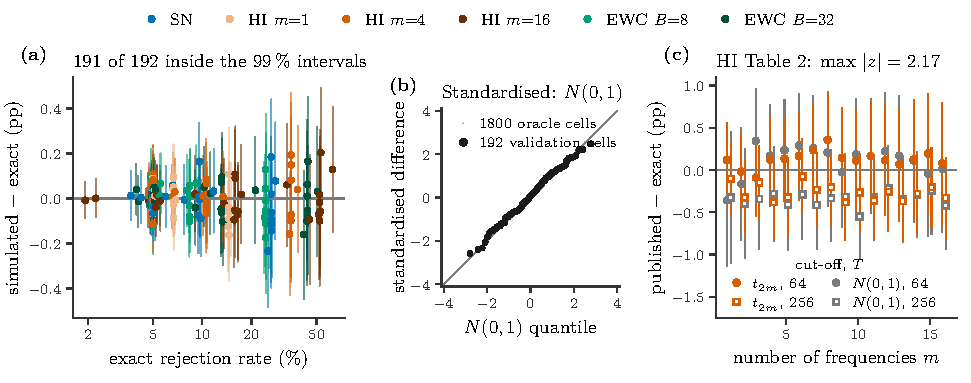
\includegraphics[width=\textwidth]{figA1_validation.pdf}
\caption{Exact finite-sample rejection rates compared with independent simulations and published rejection frequencies.}\label{fig:validation}
\end{figure}

Panel~(a) of \cref{fig:validation} shows $99\,\%$ Wilson intervals from $200\,000$ simulations per cell.
Panel~(b) compares standardised simulation errors with normal quantiles. In panel~(c), filled and open points
denote sample sizes 64 and 256; bars span two standard errors.

\paragraph{Code architecture} The package \texttt{code/p3} contains \texttt{gram.py} (closed-form cosine Gram matrices in double precision), \texttt{lowrank.py} (certified fixed-$m$ and EWC limits in Arb ball arithmetic), \texttt{certify.py} (certified distribution function of $T_H$ via adaptive complex ball quadrature and tilted midpoint cross-check), \texttt{finite\_n.py} (Cholesky-free Woodbury exact finite-sample laws, circulant-embedding sampler, local Whittle, demeaned exact local Whittle, ADG-MAC and rate-free subsampling) and \texttt{laws.py} (Imhof, Ruben and reference laws). \texttt{code/experiments} provides one driver per experiment (\cref{tab:experiments}); \texttt{code/figures} contains one script per figure, typeset with the manuscript preamble; \texttt{code/manuscript/make\_numbers.py} generates every macro and table body directly from \texttt{results/} and \texttt{literature/} and halts with a non-zero exit code if any input is missing or any internal consistency check fails.

\begin{table}[tbp]\centering\footnotesize
\caption{Experiments, outputs and scripts for reproducing the numerical results.}\label{tab:experiments}
\begin{tabular}{@{}l>{\raggedright}p{0.50\textwidth}>{\raggedright\arraybackslash}p{0.33\textwidth}@{}}\toprule
experiment & script & content\\\midrule
E0, E0d & \texttt{e0\_anchors.py, e0d\_revalidate.py} & $H=\frac12$ anchors, gate G0; part (d) with the final certificate\\
E1, E1b & \texttt{e1\_benchmark\_J.py, e1b\_nodes.py} & truncation benchmark, node counts\\
E2, E2b, E2r & \texttt{e2\_production\_sn.py, e2b\_production\_fixed.py, e2r\_revalidate.py} & certified critical values; recomputation with the final certificate\\
E3 & \texttt{e3\_finite\_n.py} & exact finite-sample sizes\\
E3b, E3c & \texttt{e3b\_mc.py, e3c\_hi2017\_table2.py, e3c\_clip\_check.py} & Monte Carlo validation, plug-in, HI reproductions; eigenvalue clipping\\
E4 & \texttt{e4\_audit.py} & audit\\
E5 & \texttt{e5\_methods.py, rq\_methods.R} & computational methods\\
E6, E6b & \texttt{e6\_naive\_size.py, e6b\_rescaled.py} & naive and rescaled sizes\\
E7, E7b, E7c & \texttt{e7\_power.py, e7b\_power\_jladder.py, e7c\_nct\_check.py} & local power; $J$ ladder; noncentral-$t$ check\\
E8, E9, E9b & \texttt{e8\_spectrum.py, e9\_surface.py, e9b\_surface\_certified.py} & spectrum, response surface, its certified held-out bound\\
E10 & \texttt{e10\_matched\_example.py} & matched finite-grid example\\
E11 & \texttt{make\_numbers.py} & independent checks (\cref{tab:reproduction})\\
E12 & \texttt{e12\_edge\_limit.py} & limit constants as $H\to1$\\
\bottomrule\end{tabular}
%
\end{table}

\paragraph{Independent verification matrix} \Cref{tab:reproduction} pairs each headline result of the main paper with an independent verification route, grouped by evidence type. Every cell is computed programmatically from the archival files in \texttt{results/}.

\begin{table}[tbp]\centering\footnotesize\setlength{\tabcolsep}{4pt}
\caption{Independent checks of numerical results by type of evidence.}\label{tab:reproduction}
\renewcommand{\arraystretch}{1.12}\begin{tabular}{@{}>{\raggedright\arraybackslash}p{0.245\textwidth}>{\raggedright\arraybackslash}p{0.205\textwidth}>{\raggedright\arraybackslash}p{0.25\textwidth}>{\raggedright\arraybackslash}p{0.24\textwidth}@{}}\toprule
Quantity & Primary computation & Independent check & Agreement\\\midrule
\multicolumn{4}{@{}l}{\textit{Enclosure compatibility}: an independent value lies inside a certified enclosure}\\[1pt]
$q_p$ of $T_{1/2}$, four levels & certified brackets, $J=16384$ & closed form \citep{AP97} & all inside\\
Cram\'er--von Mises law, three levels & certified bridge engine, $J=4096$ & closed-form quantiles & all inside\\
fixed smoothing at $H=\frac12$, $m\le16$, $B\le32$ & certified Ruben series & Student $t$ and $F$ laws & all inside\\
T1, T2: fixed smoothing, $H=0.8$ & certified Ruben series & Imhof (three codes), Ruben (double) & all inside; Davies $4.1\times10^{-11}$ outside\\
T4: $F_{0.75}$ at its $95\,\%$ point & certified, $J=16384$ & Imhof, $J=512$, remainder by its mean & inside; error $\le$ $9.5\times10^{-9}$\\
\addlinespace[4pt]
\multicolumn{4}{@{}l}{\textit{Independent implementation}: the same quantity from separate code or another algorithm}\\[1pt]
closed forms at $H=\frac12$ ($T_{1/2}$; Cram\'er--von Mises) & characteristic functions (mpmath) & Imhof over the explicit eigenvalues & $\ge14.5$; $\ge12.1$ digits\\
T3: exact law of $T_n$, $n=1000$ & Cholesky-free one-eigh (Proposition~7(b)) & Imhof, Davies, gx2 on the ratio form & $\le$ $1.9\times10^{-11}$\\
exact size of $T_n$, fGn, $n\le128$ & Woodbury inversion (Proposition~7(b)) & $30$-digit Imhof (independent code) & max $|A-B|=$ $6.7\times10^{-14}$\,pp\\
local power at $H=\frac12$, fixed smoothing & noncentral Imhof (Proposition~9) & noncentral Student $t$ & $\le$ $2.3\times10^{-13}$, 610 cells\\
\addlinespace[4pt]
\multicolumn{4}{@{}l}{\textit{Asymptotic consistency}: exact finite-sample or near-edge values approach the certified limit}\\[1pt]
$q_{0.95}$ at $H=0.99$ & certified limit & exact law, fGn, $n=128$ & size $5.000039$\,\%\\
naive size at $H=0.9$, $0.99$ & certified limits & exact law, fGn, $n=128$ & $6.9\times10^{-5}$; $9.2\times10^{-6}$\,pp\\
$(1-H)\,q_{0.95}(H)$, $H\to1$ & certified, $H=0.98$, $0.99$, extrapolated & $C_{0.95}$ of Proposition~6 & $0.04$\,\% relative\\
\addlinespace[4pt]
\multicolumn{4}{@{}l}{\textit{Probabilistic check}: simulation against exact values}\\[1pt]
finite-sample rates (Section~4) & exact laws & simulation, $R=200\,000$, 192 cells & 191 inside $99\,\%$ intervals\\
oracle rates, estimated-$H$ study & exact laws, true $H$ & simulation, 1\,800 cells & 98.9\,\% inside $99\,\%$ intervals\\
\citet[Table~2]{HI17} & exact finite-$T$ laws & their simulation & max $|z|=2.17$, 64 cells\\
\addlinespace[4pt]
\multicolumn{4}{@{}l}{\textit{Convergence check}: refinement of a discretisation parameter}\\[1pt]
Bartlett/SN local power & $J=512$ & $J=256$ and $1024$ & $\le$ $9.0\times10^{-9}$; $\le$ $1.1\times10^{-9}$\\
enclosure width of $F_H$ & $J=512,\dots,8192$ & rate $J^{-1/2-2H}$ (Proposition~11) & slopes within $0.05$\\
\addlinespace[4pt]
\multicolumn{4}{@{}l}{\textit{Cross-route verification}: independent inversion routes and deterministic re-runs}\\[1pt]
T4 certified $F_{0.75}(q_{0.95})$, $J=16384$ & adaptive complex quadrature (\texttt{acb.integral}) & tilted midpoint Poisson sum & nested overlap; width $1.87\times10^{-8}$\\
certified $q_p(H)$, 300 brackets & ball-arithmetic certificate (Appendix~B) & full independent re-certification & all 300/300 confirmed\\
\bottomrule\end{tabular}
%
\end{table}

\paragraph{Software and numerical safeguards} All files are archived in \texttt{CosCert\_code\_and\_data.zip} and at \url{https://github.com/EslamAhmedGaber/CosCert}. Computations use Python~3.12 with NumPy, SciPy, mpmath and \texttt{python-flint} (Arb), plus R~4.5 with \texttt{CompQuadForm}, \texttt{momentchi2} and \texttt{survey} and the Python package \texttt{gx2} for Section~8.2. Exact package versions are recorded in \texttt{ENVIRONMENT.json} and SHA-256 checksums of all result files in \texttt{results/SHA256SUMS.txt}. In the exact finite-sample laws (Proposition~7(b)), floating-point rounding over the \pthree{clip-ncells} design cells produced at most \pthree{clip-max} tiny negative eigenvalue per cell (in \pthree{clip-nwith} cells), of magnitude at most \pthree{clip-rel} of the largest eigenvalue, which is clipped to zero; ARFIMA$(1,d,0)$ autocovariances are truncated where the analytical remainder is below \pthree{arfima-trunc} of $\gamma(0)$.

\bibliographystyle{elsarticle-num-names}
\bibliography{references}
\end{document}
